\documentclass[twoside,a4paper,11pt]{memoir}
\usepackage{a4}
\usepackage{times}
\usepackage{pslatex}
\usepackage{url}
\usepackage{mscthesis}
\usepackage{lipsum} % standard filler text, only needed for demo

% %% The package 'algorithm' is useful, but incompatible with memoir.
% %% Cor-Paul Bezemer / http://homes.esat.kuleuven.be/~dvherten/esatthesis.html
% %% suggest the following fix:
\let\newfloat\undefined \usepackage{algorithmic} 
\usepackage{algorithm}

% Graphics setup for PDF builds.
% Avoid forcing the dvips driver so PNG figures in figures/ load correctly.
\usepackage{graphicx}
\usepackage{color}
\graphicspath{{figures/}{img/}}

\usepackage{hyperref}
\usepackage{etoolbox}
\usepackage{amsmath}
\usepackage{amssymb}

% Used in the bibliography to enable \citeauthor{citation}
\usepackage[numbers]{natbib}

% Ensure that urls longer than the page width are broken up
% Based on the answer of StackOverflow user "xamde":
% https://tex.stackexchange.com/a/10401/155506
\expandafter\def\expandafter\UrlBreaks\expandafter{\UrlBreaks%  save the current one
  \do\a\do\b\do\c\do\d\do\e\do\f\do\g\do\h\do\i\do\j%
  \do\k\do\l\do\m\do\n\do\o\do\p\do\q\do\r\do\s\do\t%
  \do\u\do\v\do\w\do\x\do\y\do\z\do\A\do\B\do\C\do\D%
  \do\E\do\F\do\G\do\H\do\I\do\J\do\K\do\L\do\M\do\N%
  \do\O\do\P\do\Q\do\R\do\S\do\T\do\U\do\V\do\W\do\X%
  \do\Y\do\Z}

%---------------------------------------------------------------------%
%                     Options                                         %    
%---------------------------------------------------------------------%

\title{Discretization Invariant and Mesh-Free \\ Operator Learning for Nuclear Reactor Modeling}
\subtitle{Version of \today}
% The final version of your thesis should typically use a different
% subtitle without the current date, for example
%\subtitle{Master's Thesis} 
% or remove the subtitle by uncommenting the following line: 
%\subtitle{}

\author{Martin Hagen}                               % CHANGE TO YOUR NAME
\authoremail{\url{m.n.hagen@student.tudelft.nl}}       % CHANGE TO YOUR EMAIL ADDRESS
%\birthplace{Weert, the Netherlands}                % CHANGE TO YOUR BIRTH PLACE
\studentid{6325203}                              % CHANGE TO YOUR STUDENT ID

% Optional for work done at a company, put this in comments if you did
% not do your thesis work at a company

% Optional (postscript) cover picture. Put this in comments when not needed.
%\coverpicture{\includegraphics[width=13cm]{img/maze.ps}}


% A copyright notice and maybe something about the cover picture
% Put in comments to get the default copyright notice
\colophon{\noindent
  \copyright{} \the\year \: \theauthor. \emph{Note that this notice is for demonstration
  purposes and that the \LaTeX{} style and document source are free to
  use as basis for your MSc thesis.} \\[1em] 
  Cover picture: A ``random'' maze generated in postscript.
}

% thesis committee:
\chair{Prof. Dr. Z. Perko, Faculty RID, TU Delft}
\supervisor{Who should I put here?, Faculty RID, TU Delft}
% The following two are optional for LaTeX (current university
% regulations state that at least one of them should be assigned)
\committeemember{Who should I put here?, Faculty RID, TU Delft}


\setcounter{tocdepth}{1}
\setsecnumdepth{subsection}
\maxsecnumdepth{subsection}

\begin{document}
\frontmatter
\thispagestyle{empty}
\maketitle                                      % for the cover page
\makeformaltitlepages{Partial differential equations (PDEs) are central to scientific computing and engineering, but high-fidelity numerical simulations are often computationally expensive. Neural operators have recently emerged as a promising approach for surrogate modeling by learning mappings between function spaces rather than finite-dimensional vectors.

A key challenge for such models is discretization invariance: the ability to produce consistent predictions when the same underlying problem is represented on different discretizations. This thesis studies this property for Fourier- and convolution-based neural operators on uniform Cartesian grids, and evaluates a geometry-aware Fourier neural operator on non-uniform point-cloud domains.

On uniform grids, the Fourier Neural Operator (FNO) and the Convolutional Neural Operator (CNO) are evaluated on Navier--Stokes and Darcy flow benchmarks through resolution-transfer experiments. The CNO shows substantially flatter loss curves across resolutions, while diagnostic experiments identify fixed-cell spatial padding as the main source of poor FNO resolution transfer in the tested implementation. Resampling inputs to a fixed internal grid largely removes this padding-induced mismatch and makes the FNO loss much more consistent across resolutions.

For non-uniform meshes, the geometry-aware Fourier Neural Operator (Geo-FNO) is evaluated on incompressible fluid flow past a cylinder and on a high-temperature gas-cooled reactor (HTGR) temperature dataset. The results show that Geo-FNO produces accurate predictions on irregular spatial representations, capturing the dominant flow and temperature structures without interpolation onto a uniform Cartesian grid. A full test of mesh-free discretization invariance would require controlled refinement of the same physical samples across multiple point-cloud discretizations.}         % for formal title pages with all info

\include{sections/preface}

\cleardoublepage\tableofcontents
\cleardoublepage\mainmatter

\chapter{\label{cha:intro}Introduction}

Partial differential equations (PDEs) are central to scientific computing and engineering because they describe how physical systems evolve. Fluid flow, heat transfer, structural deformation, neutron transport, and porous-media flow can all be formulated through PDEs. In nuclear engineering in particular, reactor analysis depends heavily on solving large coupled PDE systems describing neutronics, thermohydraulics, heat conduction, and structural behavior.

Classical numerical methods such as finite difference, finite element, and finite volume methods provide accurate solutions to these problems, but they are often computationally expensive. High-fidelity simulations may require fine spatial discretizations, long transient integrations, or repeated solves under varying parameters. This becomes particularly challenging in applications such as optimization, uncertainty quantification, design studies, and real-time decision support, where the same governing equations must be solved many times under different conditions.

This motivates the use of learning-based surrogate models; machine learning models trained to emulate the behavior of expensive numerical solvers while producing predictions at orders of magnitude lower computational cost \cite{ml-good}. Once trained, such models can provide rapid evaluations of complex physical systems, making them attractive for engineering workflows where repeated PDE solves are the primary computational bottleneck.

However, standard machine learning models are typically formulated as mappings between finite-dimensional vectors. A conventional neural network learns a mapping of the form
\[
x \mapsto y,
\]
where both the input and output are fixed-dimensional vectors. PDE problems, however, are naturally function-to-function problems. The input may be an initial condition, boundary condition, forcing term, or material coefficient field, while the output is itself a function such as a pressure field, temperature distribution, or velocity field. The object being learned is therefore not a vector-valued map, but an operator between function spaces.

Neural operators were introduced to address this setting directly. Rather than learning a mapping between discretized vectors, they aim to approximate the underlying continuous solution operator of a PDE. Instead of learning a map tied to one specific discretization, the model approximates the operator itself, allowing the same learned model to be evaluated across multiple discretizations of the same underlying problem. This property is one of the main distinctions between neural operators and standard surrogate models.

This property is commonly referred to as discretization invariance. Informally, a discretization-invariant model should produce consistent predictions when the same underlying function is represented on different discretizations, provided those discretizations sufficiently resolve the relevant physics. In this sense, the model depends on the underlying continuous object rather than on the particular grid used to represent it.

Discretization invariance is one of the central criteria used to evaluate neural operators in practice. In this thesis, it is examined directly on uniform Cartesian grids through resolution-transfer experiments, and later discussed in the context of non-uniform meshes and point clouds, where the notion of discretization is less straightforward and does not admit the same type of evaluation.

This motivates the two-part structure of this thesis. The first part investigates discretization invariance on uniform Cartesian grids using two important neural operator architectures: the Fourier Neural Operator (FNO) and the Convolutional Neural Operator (CNO). These models are evaluated on Navier--Stokes and Darcy flow benchmarks to study how architectural choices affect robustness under resolution transfer.

The second part considers mesh-free operator learning on irregular domains using the geometry-aware Fourier Neural Operator (Geo-FNO). The goal here is to evaluate whether operator learning can be performed directly on non-uniform meshes while preserving physically meaningful predictions. This is studied on both a standard fluid benchmark involving incompressible flow past a cylinder and a reactor-relevant high-temperature gas-cooled reactor (HTGR) temperature dataset.

In addition to evaluating these architectures, this thesis also investigates practical implementation issues that affect operator learning on irregular domains. In particular, a bug in the original Geo-FNO implementation was identified and corrected, removing a persistent seam artifact that appeared across all tested datasets and significantly improving predictive accuracy. The proposed fix was later incorporated into the official implementation.

The central research question investigated in this thesis is:

\begin{itemize}
    \item To what extent can Fourier- and convolution-based neural operator methods provide discretization-robust surrogate models for PDE-based data on both uniform grids and non-uniform point clouds?
\end{itemize}

This is further divided into the following sub-questions:

\begin{itemize}
    \item To what extent do FNO and CNO generalize across grid resolutions on uniform-grid PDE benchmarks?
    
    \item How effectively does Geo-FNO enable Fourier-based operator learning on non-uniform point-cloud data?
    
    \item What limitations arise when applying Geo-FNO to reactor-relevant data defined on irregular meshes?
\end{itemize}

The main contributions of this thesis are threefold. First, it provides a systematic comparison of FNO and CNO under resolution transfer, showing how spectral truncation, fixed internal resampling, and aliasing control affect discretization robustness. Second, it evaluates Geo-FNO on irregular-domain problems and clarifies how discretization invariance should be interpreted in the mesh-free setting. Third, it demonstrates the applicability of neural operators to reactor-relevant non-uniform data while identifying both practical limitations of the current datasets and implementation issues that arise in real mesh-free applications.

The remainder of this thesis is structured as follows. Chapter~\ref{cha:background} introduces the theoretical background of operator learning, discretization invariance, and the neural operator architectures studied in this work. Chapter~\ref{cha:method} describes the datasets, training procedures, and experimental design. Chapter~\ref{cha:uniform-results-discussion} presents the uniform-grid experiments and discusses the behavior of FNO and CNO under resolution transfer. Chapter~\ref{cha:non-uniform-results-discussion} presents the mesh-free experiments with Geo-FNO on irregular domains and discusses their implications for discretization invariance on non-uniform meshes. Finally, Chapter~\ref{cha:conclusion} summarizes the conclusions of the thesis and outlines directions for future work.
 
\chapter{\label{cha:background}Background \& Theory}

\section{Operator Learning}\label{sec:operator-learning}

Operator learning refers to the use of neural networks to approximate mappings between function spaces, rather than between finite-dimensional vectors as is done for classical neural network approaches \cite{neural-operators}. This setting arises naturally in scientific computing, where many problems can be formulated in terms of operators acting on functions.

A particularly important example is the solution operator of a parametric partial differential equation (PDE). Consider a PDE of the form:
\begin{equation}
\mathcal{N}(a, u)(x) = f(x), \quad x \in \Omega, \qquad u(x) = 0, \quad x \in \partial \Omega,
\end{equation}
where $\Omega \subset \mathbb{R}^d$ is a bounded domain, $\mathcal{N}$ is an operator, $a$ is an input function, $f$ is an external term like a forcing term, and $u$ is the solution.

The corresponding solution operator is defined as:
\begin{equation}
\mathcal{G}(a)(x) = u(x),
\end{equation}
which maps an input function $a$ to the solution $u$. The goal of operator learning is to approximate this mapping directly using surrogate modeling. 

Let $\mathcal{A}$ and $\mathcal{U}$ denote appropriate function spaces for the input and output, respectively. Given a dataset of input-output pairs:
\begin{equation}
\{(a_j, u_j)\}_{j=1}^{N_{\text{data}}}, \quad u_j = \mathcal{G}(a_j),
\end{equation}
where the inputs $a_j$ are sampled from a distribution $\mu$ over $\mathcal{A}$, the objective is to learn a parametric approximation $\mathcal{G}_\theta : \mathcal{A} \to \mathcal{U}$ by minimizing the expected error
\begin{equation}
\mathbb{E}_{a \sim \mu} \left[ \| \mathcal{G}(a) - \mathcal{G}_\theta(a) \|_{\mathcal{U}}^2 \right],
\end{equation}
which in practice is approximated by the empirical loss over the dataset.

A common theoretical formulation of neural operators represents each layer as
\begin{equation}
    \label{eq:og-formulation}
v_{\ell+1}(x)=\sigma\left(Wv_\ell(x)+\int_{\Omega}\kappa(x,y)v_\ell(y)\,dy\right),
\end{equation}
where $v_\ell(x)$ denotes the latent feature representation at spatial location $x$ in layer $\ell$, $W$ is a pointwise channel-mixing operator, $\kappa(x,y)$ is a learned kernel describing interactions between spatial locations $x$ and $y$, and $\sigma$ is a nonlinear activation function \cite{neural-operators}. Unlike standard neural network layers, which operate on fixed finite-dimensional vectors, this formulation acts on functions defined over a continuous domain through a global integral operator. In principle, this allows the learned mapping to depend on the underlying continuous function rather than on a specific discretization. In practice, however, neural operators are always trained on discretized samples of functions, and different architectures approximate this idealized formulation to different degrees.

A key distinction from standard learning problems is therefore that the objects of interest are continuous functions rather than finite-dimensional vectors, even though they are only observed through discrete samples. The learning problem is formulated at the level of a continuous operator, while training and inference are performed on discretized representations. Understanding what information about a function is preserved under discretization is therefore central to understanding discretization invariance in neural operators.

\subsection{Bandlimitedness and Continuous--Discrete Equivalence}\label{sec:bandlimitedness}

A central question in operator learning is what information about a continuous function is preserved when it is represented through discrete samples. Sampling theory provides a framework for answering this question, by characterizing when a function can be uniquely reconstructed from its values on a discrete grid.



Let $f \in L^2(\mathbb{R})$ be a square-integrable function with Fourier transform $\hat{f}$. The function is said to be bandlimited with bandlimit $\Omega > 0$ if its Fourier transform is supported only on a finite interval:
\begin{equation}
\mathrm{supp}(\hat{f}) \subset [-\Omega, \Omega].
\end{equation}

The Whittaker-Shannon sampling theorem states that a bandlimited function can be exactly reconstructed from its values on a uniform grid, provided the sampling rate is sufficiently high \cite{signals-and-systems}. Specifically, if the function is sampled at points $\{f(nT)\}_{n \in \mathbb{Z}}$, then exact reconstruction is possible if
\begin{equation}
\frac{1}{T} \geq 2\Omega,
\end{equation}
where $1/T$ is the sampling frequency and $2\Omega$ is called the Nyquist rate.

Under this condition, the function can be reconstructed via the interpolation formula
\begin{equation}
f(x) = \sum_{n \in \mathbb{Z}} f(nT)\,\mathrm{sinc}\left(\frac{x - nT}{T}\right),
\end{equation}
where $\mathrm{sinc}(x) = \frac{\sin(\pi x)}{\pi x}$.

This result establishes a form of continuous--discrete equivalence: if a function is bandlimited and sampled above the Nyquist rate, then its discrete samples contain all the information required to reconstruct the original function. In this case, the discretization is effectively lossless.

However, if the sampling rate is below the Nyquist rate, this equivalence breaks down. Different continuous functions can then produce the same values at the sampled points, so the original function can no longer be uniquely reconstructed from the discrete data. In Fourier terms, the unresolved high-frequency components do not remain separate from the resolved part of the spectrum. Instead, they appear on the sampled grid as lower-frequency components.

This misrepresentation of unresolved high-frequency content as lower-frequency content is known as aliasing. Intuitively, aliasing occurs when the function oscillates too rapidly relative to the spacing between sample points. The grid cannot represent this oscillation as a distinct high-frequency component, so it appears in the sampled data as a lower-frequency oscillation.

Figure~\ref{fig:aliasing} illustrates this effect. The blue curve represents a high-frequency signal, while the red curve is a lower-frequency function passing through the same sampled points. Since the sampled representation contains only the values at the black dots, both continuous functions correspond to the same discrete data. If the lower-frequency curve lies inside the range of frequencies that the grid can represent while the high-frequency curve lies outside it, the sampled representation interprets the high-frequency signal as its lower-frequency alias.

\begin{figure}
    \centering
    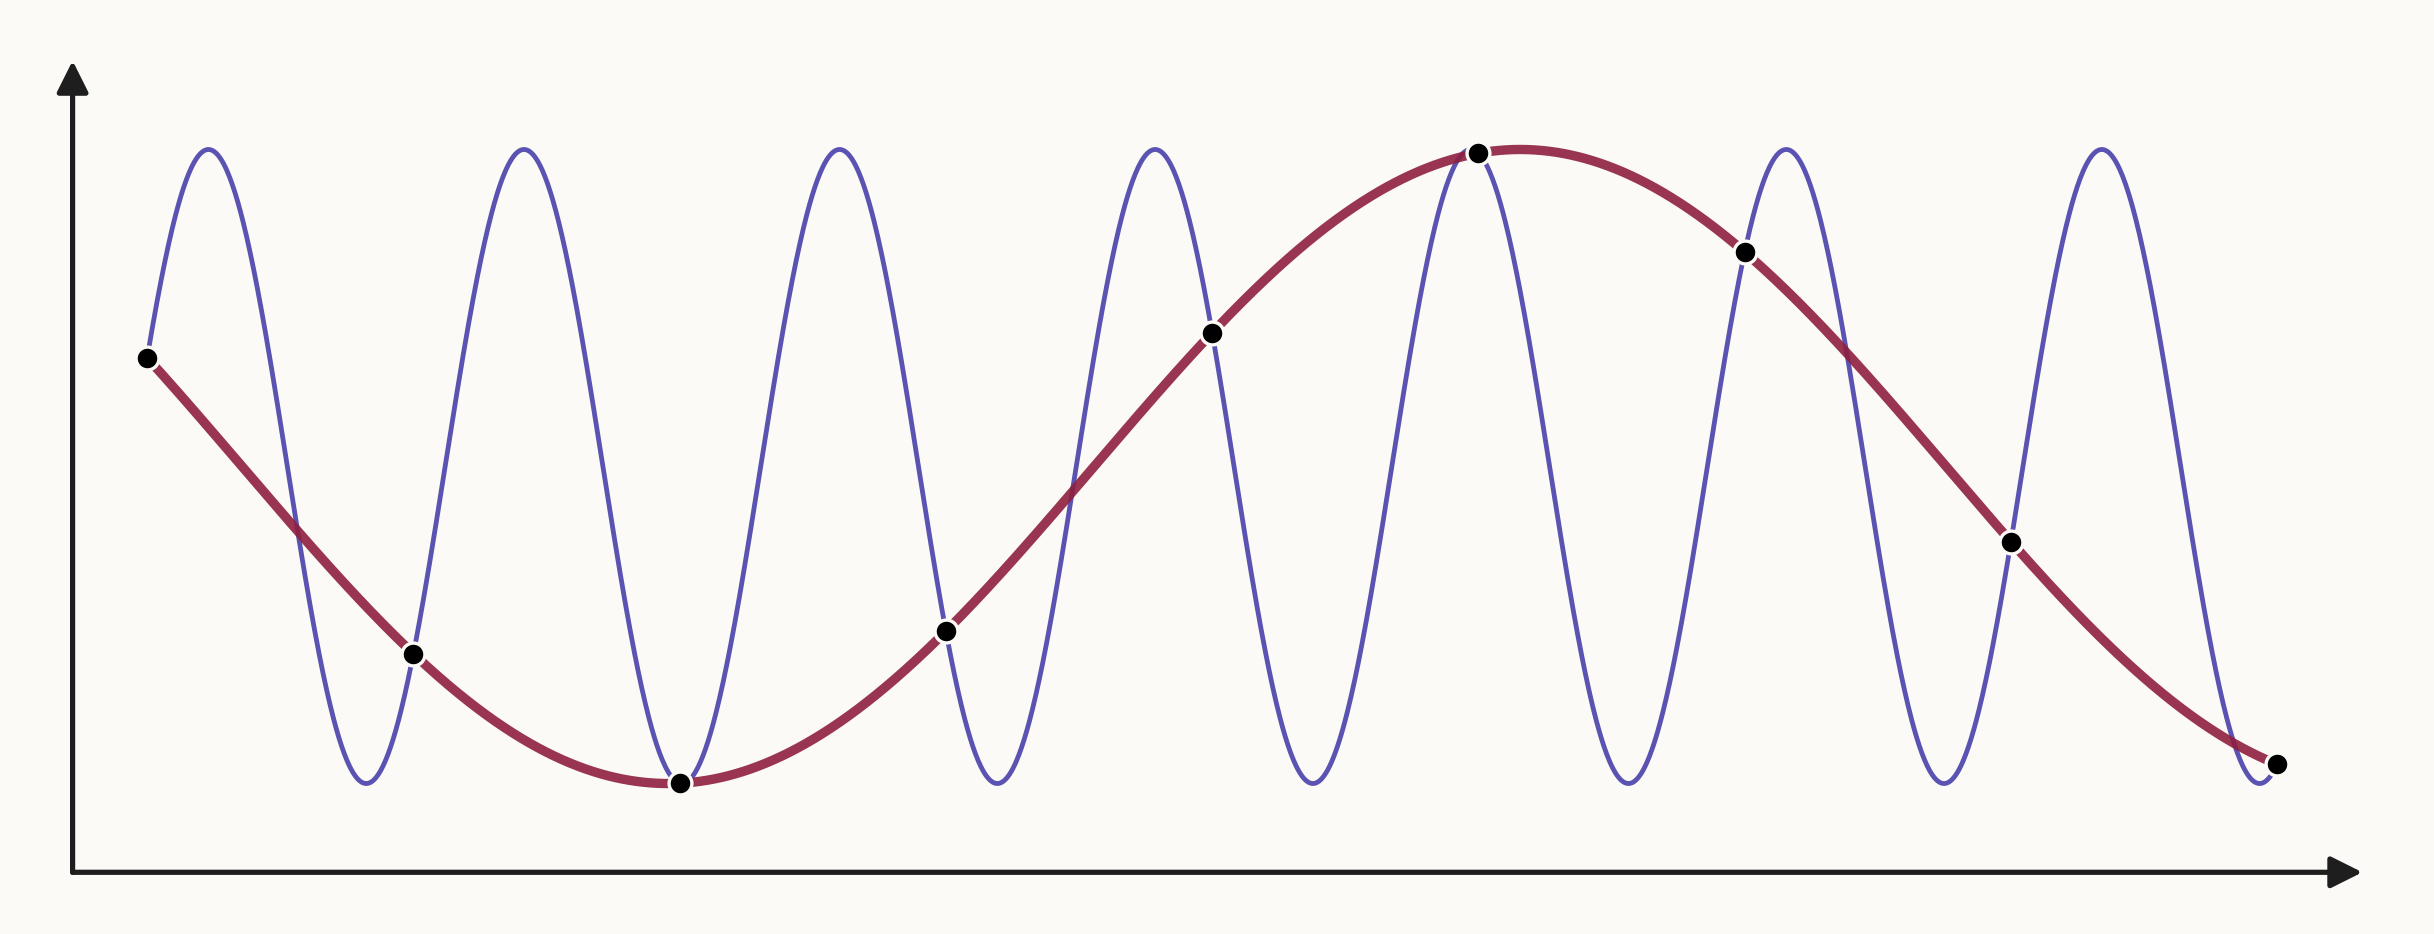
\includegraphics[width=0.8\textwidth]{figures/aliasing.png}
    \caption{\label{fig:aliasing} An illustration of aliasing. The blue curve represents a high-frequency signal, while the red curve is a lower-frequency function that passes through the same sampled points (black dots). Since both functions agree at the sampling locations, the discrete representation cannot distinguish between them.}
\end{figure}

From a Fourier perspective, once the sampling spacing \(T\) has been fixed, the grid has a maximum representable angular frequency. This is the Nyquist limit,
\begin{equation}
\omega_N = \frac{\pi}{T},
\end{equation}
where \(T\) is the spacing between sample points. Equivalently, \(\omega_N\) is half the sampling angular frequency \(2\pi/T\). Frequencies satisfying
\begin{equation}
|\omega| \leq \omega_N
\end{equation}
can be represented uniquely on the sampled grid, while frequencies above this limit cannot.

Consider a sinusoidal component
\begin{equation}
f(x) = \sin(\omega x).
\end{equation}
Sampling this function at points \(x_n = nT\) gives
\begin{equation}
f(nT) = \sin(\omega nT).
\end{equation}
The samples are unchanged when the frequency is shifted by an integer multiple of the sampling angular frequency \(2\pi/T\). Since \(2\omega_N = 2\pi/T\), frequencies of the form
\begin{equation}
\omega - 2k\omega_N, \qquad k \in \mathbb{Z},
\end{equation}
produce the same discrete oscillation after sampling. The represented frequency is obtained by choosing \(k\) so that the shifted frequency lies inside the Nyquist interval:
\begin{equation}
-\omega_N \leq \omega - 2k\omega_N \leq \omega_N.
\end{equation}
For a real-valued sinusoid, this is often reported as the non-negative aliased frequency
\begin{equation}
\omega_{\mathrm{alias}} = |\omega - 2k\omega_N|,
\end{equation}
with \(k\) chosen such that
\begin{equation}
0 \leq \omega_{\mathrm{alias}} \leq \omega_N.
\end{equation}

This mapping of frequencies outside the Nyquist interval back into the representable band is called folding. Sampling below the Nyquist rate therefore does not simply remove all frequency content above \(\omega_N\). Instead, unresolved high-frequency components are folded into lower represented frequencies. If several continuous Fourier components fold onto the same represented frequency, their complex Fourier coefficients contribute to the same discrete mode. Depending on their phases, these contributions may reinforce or partially cancel. The sampled data therefore contains a distorted spectrum in which unresolved high-frequency content contaminates modes that appear to be lower frequency.

The consequence is that information above the Nyquist limit is irreversibly lost as distinct high-frequency information. Once aliasing has occurred, the sampled data no longer contains enough information to determine whether a represented low-frequency mode came from a true low-frequency component, from unresolved high-frequency content, or from a combination of both. No learning algorithm can reconstruct frequency content that is absent from the discretized data, regardless of model complexity or architecture \cite{bartolucci-discretization-invariance}.

In the context of neural operators, aliasing can arise in two distinct ways. The first occurs during discretization of the original continuous function, when the sampling rate is insufficient to resolve the underlying frequency content. This form of aliasing is a property of the data representation itself and cannot be corrected after sampling has taken place. A second form of aliasing can occur inside the neural operator architecture. Nonlinear operations applied to bandlimited representations generate new higher-frequency components that may lie above the Nyquist limit of the internal discretization used by the model. If these components are not explicitly removed, they fold into the representable frequency range and alter the resolved modes. This architectural form of aliasing can therefore occur even when the original sampled input data is sufficiently resolved.


\subsection{Discretization Invariance}\label{sec:discretization-invariance}

The discussion in Section \ref{sec:bandlimitedness} shows that learning from discretized data is fundamentally constrained by the information preserved under sampling. Even if a model is intended to approximate a continuous operator, it is trained and evaluated on finite representations of functions. This raises the question of whether the learned model depends only on the underlying function, or also on the particular discretization used to represent it.

The desired property is referred to as discretization invariance. Informally, a discretization\hyp{}invariant model should produce consistent predictions when the same underlying function is represented on different grids, provided those discretizations sufficiently resolve the relevant features of the problem.

In practice, discretization invariance is most naturally interpreted for functions represented on uniform Cartesian grids, where resolution can be clearly defined through grid spacing. In this setting, it refers to the ability of a model trained at one resolution to make accurate predictions of the same underlying problem represented at other resolutions.

A widely used definition of neural operators is given by Kovachki et al. \cite{neural-operators}, stating that a neural operator should satisfy three key properties:

\begin{enumerate}
    \item \textbf{Discretization flexibility:} the model can accept inputs defined on arbitrary discretizations of the domain.
    
    \item \textbf{Pointwise evaluation:} the model can be evaluated at arbitrary output locations.
    
    \item \textbf{Continuum consistency:} as the discretization is refined, the learned operator converges to the underlying continuous operator being approximated.
\end{enumerate}

These properties formalize the idealized objective that a neural operator should approximate a mapping between functions. In this view, the learned operator should primarily depend on the underlying continuous object rather than on the particular resolution, ordering, or structure of the discretization used to represent it. In practice, however, many architectures still retain a significant dependence on the representation used during training.

This dependence becomes visible when the discretization is changed. If refining or otherwise changing the discretization changes the model output, the model is tied to the training representation rather than to the operator itself. As a result, performance may degrade significantly when evaluated on different resolutions or different discretizations of the same problem. This phenomenon is referred to as discretization mismatch \cite{gao-discretization-invariance}.

Discretization invariance is therefore a central criterion for evaluating neural operator architectures. In this thesis, it is used both as a theoretical concept and as an empirical measure for comparing models across changes in resolution.

\section{Fourier Neural Operator -- FNO}\label{sec:fno}

The Fourier Neural Operator (FNO), introduced by Li et al. \cite{li2021fno}, was the first major neural operator architecture to demonstrate strong performance on large-scale PDE learning problems and remains one of the most influential models in operator learning. Its success established neural operators as a practical alternative to classical numerical solvers and motivated much of the subsequent development in the field \cite{fno-explained}, including architectures such as the Convolutional Neural Operator (CNO) and geometry-aware Fourier Neural Operator (Geo-FNO).

\begin{figure}
    \centering
    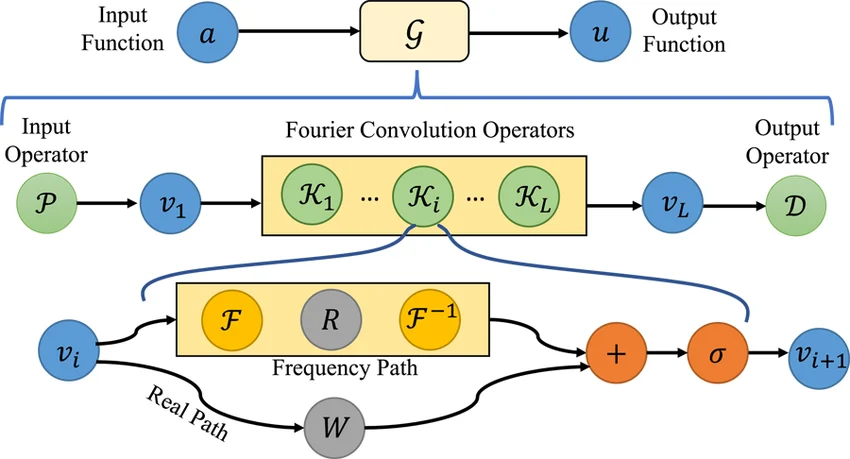
\includegraphics[width=0.8\textwidth]{figures/fno_figure.png}
    \caption{\label{fig:fno_architecture} The architecture of the Fourier Neural Operator (FNO), showing the lifting layer, repeated Fourier layers consisting of spectral convolution and pointwise channel mixing, and the final projection layer. \cite{fno-figure}.}
\end{figure}

The central idea of the FNO is to learn the solution operator in Fourier space. The model performs global convolution by transforming the input field into its Fourier representation, applying learned transformations to the Fourier coefficients, and transforming the result back to the spatial domain.

Figure~\ref{fig:fno_architecture} illustrates the architecture of the FNO. The model approximates the solution operator
\[
\mathcal{G}: a \mapsto u ,
\]
where $a$ is the input function and $u$ is the corresponding solution field. The full network consists of three main components: an input lifting operator, a sequence of Fourier layers, and an output projection operator.

The lifting operator maps the input field into a higher-dimensional latent representation,
\begin{equation}
\mathcal{P}: a(x) \rightarrow v_1(x),
\end{equation}
where $v_1(x)$ contains a larger number of feature channels than the original physical field. This allows the subsequent Fourier layers to operate in a richer latent space rather than directly on the low-dimensional physical variables.

The core of the architecture is the Fourier layer. Given an intermediate representation $v_l(x)$, each layer updates the features according to
\begin{equation}
v_{l+1}(x)
=
\sigma
\left(
Wv_l(x)
+
\mathcal{K}(v_l)(x)
\right),
\end{equation}
where $\mathcal{K}$ is the spectral convolution operator, $W$ is a pointwise linear transformation, and $\sigma$ is a nonlinear activation function.

The spectral convolution operator is implemented by first applying a Fourier transform to the input features that acts per channel, followed by truncation to a fixed number of low-frequency Fourier modes. For each retained mode, learned complex-valued weight matrices are applied to mix information across feature channels in frequency space. Finally, an inverse Fourier transform maps the result back to the spatial domain,
\begin{equation}
\mathcal{K}(v_l)
=
\mathcal{F}^{-1}
\left(
R \cdot \mathcal{F}(v_l)
\right),
\end{equation}
where $R$ denotes the learned complex weights acting on the retained modes as shown in Figure \ref{fig:fno_architecture}.

This frequency-space formulation is what distinguishes the FNO from standard convolutional architectures. Instead of learning kernels tied to a fixed spatial stencil, the model learns transformations of Fourier modes, which correspond to global basis functions spanning the entire domain.

Alongside the spectral path, the term $Wv_l(x)$ provides a local pointwise linear transformation in physical space. This is a channel-mixing operator analogous to a $1 \times 1$ convolution. It allows the model to incorporate local, pointwise corrections that cannot be represented by the truncated set of retained Fourier modes. Note that although $W$ and $\mathcal{K}$ are linear operations, the nonlinearity $\sigma$ allows the model to learn nonlinearities.

After several Fourier layers, the projection operator maps the final latent representation back to the physical output space,
\begin{equation}
\mathcal{D}: v_L(x) \rightarrow u(x),
\end{equation}
producing the predicted solution field.

\subsection{Strengths}

One of the main strengths of the FNO is its ability to capture global dependencies efficiently. Since Fourier modes are global basis functions, modifying a single coefficient influences the solution across the entire domain. This gives the model a global receptive field in every layer, making it particularly well suited for PDEs whose solution operators exhibit long-range interactions.

A second major advantage is computational efficiency. As discussed in Section~\ref{sec:operator-learning}, the theoretical neural operator formulation in Equation~\ref{eq:og-formulation} defines global interactions across the spatial domain through an integral operator. Directly evaluating the pairwise interactions implied by this formulation requires quadratic complexity in the number of spatial points $n$. The FNO avoids this cost by parameterizing the operator in Fourier space. By the convolution theorem, convolution in physical space is equivalent to pointwise multiplication in Fourier space. The spectral convolution can therefore be computed efficiently using the Fast Fourier Transform (FFT), reducing the computational complexity to
\begin{equation}
\mathcal{O}(n \log n),
\end{equation}
which makes large-scale operator learning computationally feasible.

The use of Fourier coefficients also provides a degree of resolution transfer across uniform Cartesian grids. Since the learned parameters act on modes rather than individual grid points, the same operator can be applied to different uniform resolutions without retraining, provided the relevant frequency content is sufficiently resolved. This makes the FNO significantly more flexible than standard convolutional networks, which are often strongly tied to the discretization used during training.

\subsection{Weaknesses}

The primary limitation of the FNO is its reliance on spectral truncation. In each Fourier layer, only a fixed number of low-frequency modes are retained, while the remaining higher\hyp{}frequency coefficients are discarded. This introduces an explicit architectural bandlimit determined by the number of retained modes.

This architectural bandlimit should be distinguished from the sampling bandlimit discussed in Section~\ref{sec:bandlimitedness}. In the sampling setting, frequencies above the Nyquist limit cannot be represented in the discretized data itself. In contrast, the FNO may discard higher\hyp{}frequency information even when those frequencies are present in the sampled input data, simply because they lie outside the retained set of Fourier modes. The architecture therefore imposes an additional spectral bottleneck beyond the limitations already introduced by discretization.

Another limitation concerns nonlinear aliasing. Pointwise nonlinear activations can generate frequency components that were not present in the input representation. If these components exceed the representable bandwidth of the discretized feature field, they cannot be resolved and instead appear as lower-frequency components through folding. This contaminates the resolved modes and can reduce the consistency of the learned representation across discretizations. 

A third important limitation is the reliance on uniform Cartesian grids. The standard FFT assumes regularly spaced points with consistent ordering, which makes the original FNO naturally suited for structured meshes but difficult to apply directly to irregular geometries or unstructured point clouds.




\section{Convolutional Neural Operator -- CNO} \label{sec:cno}

\subsection{Architecture}

\begin{figure}
    \centering
    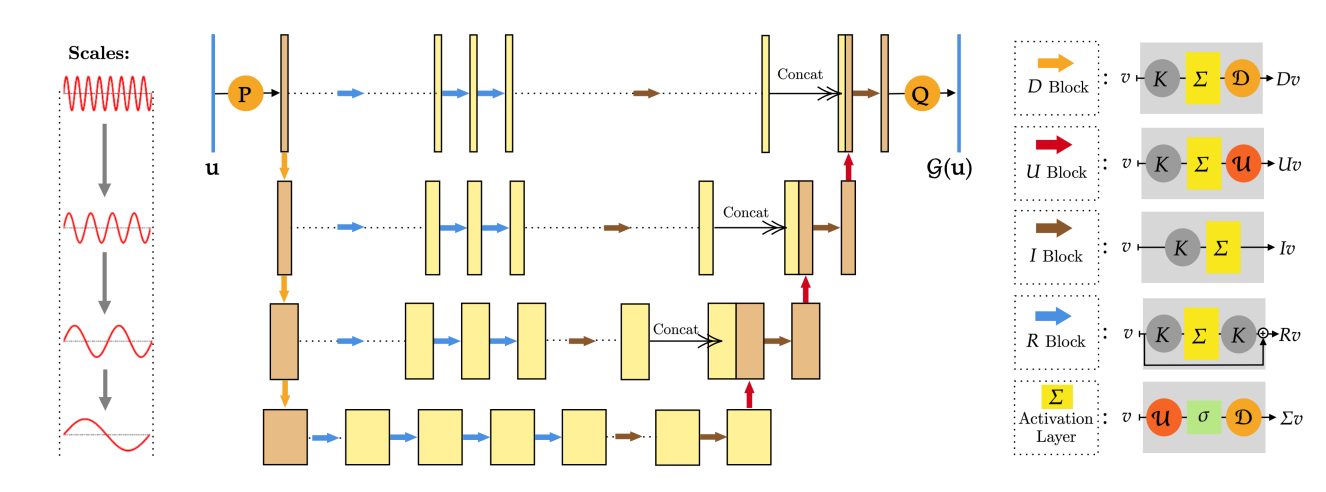
\includegraphics[width=0.8\textwidth]{figures/cno_figure.png}
    \caption{\label{fig:cno-architecture} The architecture of the Convolutional Neural Operator (CNO) \cite{cno}, showing the lifting operator $P$, projection operator $Q$, and the central U-shaped neural operator structure. The network combines downsampling ($D$-blocks), upsampling ($U$-blocks), residual blocks ($R$-blocks), and invariant blocks ($I$-blocks) across multiple spatial scales, with skip connections and concatenation used to preserve multiscale information. Anti-aliased downsampling and upsampling ensure resolution-invariant feature propagation across discretizations.}
\end{figure}

The Convolutional Neural Operator (CNO), introduced by Raonic et al. \cite{cno}, extends the classical U-Net architecture \cite{U-net} to the operator learning setting. U-Nets and related convolutional neural networks have been highly successful in fields such as image processing and segmentation due to their ability to efficiently capture local spatial structure through convolutional kernels \cite{U-net}. The CNO adopts this encoder--decoder structure while introducing several modifications aimed at satisfying the discretization invariance requirements discussed in Section~\ref{sec:discretization-invariance}.

Unlike the Fourier Neural Operator, which learns global interactions through Fourier modes, the CNO is built on standard convolutions in physical space. A convolutional kernel acts on a local neighborhood of points, producing a local operator rather than a global spectral one. This makes the model structurally similar to standard convolutional neural networks, but introduces an important challenge for operator learning: the physical meaning of a fixed kernel depends on the discretization.

For example, a $3 \times 3$ kernel applied on a coarse grid covers a much larger physical region than the same kernel on a fine grid. As a result, a standard CNN or U-Net is not naturally discretization invariant, since changing the resolution changes the effective operator being learned.

To address this, the CNO uses a multi-scale encoder--decoder architecture together with an initial resampling step onto a fixed internal resolution. Figure~\ref{fig:cno-architecture} illustrates the overall structure. After the initial resampling, the input is passed through a lifting layer, which maps the physical input field into a higher-dimensional feature space. This serves the same purpose as in the FNO, allowing the operator to be learned in a richer latent representation.

The lifted representation then enters the encoder, where it passes through a sequence of convolutional blocks. Each block consists of a convolution followed by a nonlinear activation. As the representation moves deeper into the encoder, the spatial resolution is progressively reduced through interpolation-based downsampling, while the number of feature channels is increased. Although the kernel size remains fixed, applying it at multiple resolutions allows the network to process information across different spatial scales.

At the coarsest level, the decoder progressively reconstructs the solution by upsampling the representation back to higher resolutions. After each upsampling step, another convolutional block is applied. Skip connections link encoder and decoder stages at matching resolutions, allowing fine-scale information from earlier layers to be reintroduced during reconstruction.

A key modification compared to a standard U-Net is the use of resampling onto a fixed internal grid before the main operator learning begins. Regardless of the input resolution, the model first interpolates the input onto the same internal discretization. This ensures that the convolutional kernels always act over the same physical scale inside the network.

This design also connects directly to the bandlimitedness discussion in Section~\ref{sec:bandlimitedness}. By choosing a fixed internal resolution, the CNO imposes an explicit bandlimit on the learned representation. Frequencies beyond this scale are removed during resampling, so the model always operates on a controlled frequency range.

A second major modification is the replacement of standard pointwise nonlinearities with the upsample--nonlinearity--downsample (UND) block. A standard pointwise activation applied directly on a finite grid is not representation-equivalent: even if the input is bandlimited, the nonlinearity generates new higher-frequency components that may lie above the Nyquist limit. These unresolved frequencies alias into lower modes, making the discrete nonlinear operator inconsistent with the corresponding continuous operator and violating the continuum consistency condition discussed in Section~\ref{sec:discretization-invariance}.

To address this, the CNO first upsamples the representation before applying the nonlinearity, creating spectral room for the newly generated frequencies to exist without immediately aliasing into the resolved modes. After the activation is applied, the representation is downsampled back to the original resolution using a low-pass filtering operation that removes the unresolved high-frequency content. Ideally, this filtering would be performed using the sinc interpolation filter implied by the Whittaker--Shannon sampling theorem, which provides exact reconstruction for bandlimited functions \cite{signals-and-systems}. In practice, this is approximated by a finite-support low-pass blur filter for computational efficiency, since exact sinc filtering is non-local and expensive to evaluate.

After the decoder stage, a projection layer maps the final latent representation back to the physical output space, producing the predicted solution field. Together, the fixed-grid resampling and the UND block are the central modifications that distinguish the CNO from a standard U-Net and make it suitable for operator learning across multiple discretizations.

\subsection{Strengths}

A major strength of the CNO is its strong local inductive bias. Since the model is built on standard convolutions in physical space, it naturally captures local interactions where the state at a point depends primarily on its immediate neighborhood. This is particularly well suited for many physical systems such as advection, diffusion, heat transfer, and turbulence-dominated flows, where local spatial structure plays a dominant role.

The encoder--decoder structure further allows the model to capture interactions across multiple physical scales. Coarse-resolution layers represent large-scale structures and long-range behavior, while fine-resolution layers preserve localized detail through skip connections. This is especially important for multiscale systems such as Navier--Stokes flow, where energy is transferred across a wide range of length scales and both global and local behavior must be represented simultaneously.

Another important advantage is robustness across resolutions. For the CNO, resampling onto a fixed internal grid is required for the convolutional kernels to retain the same physical meaning when the input resolution changes. Otherwise, a fixed-size kernel would correspond to different physical length scales on different grids. This consistency comes at the cost of an interpolation step, which is not lossless and may introduce artifacts or remove high-frequency information. The advantage of the CNO is therefore that it trades interpolation error for a fixed internal representation on which the learned convolutional operator can act consistently. When the internal resolution is sufficiently high for the relevant features of the problem, this trade-off can lead to substantially more stable behavior under resolution transfer.

The explicit treatment of bandlimiting also provides an important advantage compared to architectures where truncation occurs only implicitly. By controlling both resampling and nonlinear aliasing through the fixed internal grid and the UND block, the CNO avoids many of the spectral artifacts associated with unresolved high-frequency content. This improves continuum consistency and makes the model much closer to satisfying the definition of a true neural operator discussed in Section~\ref{sec:discretization-invariance} and in the work of Bertolucci et al. \cite{bartolucci-discretization-invariance}.

\subsection{Weaknesses}

A practical limitation of the CNO is its dependence on the chosen internal resolution. The resampling step improves consistency by enforcing a fixed internal representation, but this resolution must be selected when the model is built and remains fixed after training. This amounts to assuming that the chosen internal grid is sufficiently fine to represent the physically relevant features of the problem. If an input or target contains structures above the Nyquist limit of the internal grid, those structures cannot be represented faithfully after resampling: they are either removed by the low-pass filtering operation or, if insufficiently filtered, aliased into lower represented modes. In this case, the model may remain stable across resolutions, but it is stable with respect to an under-resolved internal representation.

This explicit truncation of high-frequency information is therefore both a strength and a weakness. While it improves robustness and discretization consistency, it can reduce accuracy for problems where sharp gradients, discontinuities, or fine-scale geometric details play a dominant role. In such cases, the CNO may sacrifice important local information in exchange for stability.

Another practical limitation is the reliance on interpolation during resampling. Both the initial resampling onto the fixed internal grid and the repeated upsampling and downsampling operations in the UND blocks introduce approximation errors. Ideally, these operations would be performed using exact sinc interpolation for bandlimited functions, but in practice finite-support approximations are used for computational efficiency, which can introduce errors.

Finally, while the CNO improves discretization invariance substantially compared to standard U-Nets, it is still not fully resolution-independent in practice. Its behavior remains tied to the chosen internal discretization, meaning that discretization robustness depends strongly on how well this internal representation matches the true frequency content of the underlying problem.


\section{Mesh-free Operator Learning and Geo-FNO}

\subsection{Motivation for Irregular Domains}

The neural operators introduced in Sections~\ref{sec:fno} and~\ref{sec:cno} assume that the input and output fields are represented on uniform Cartesian grids. While this assumption is convenient for both Fourier-based and convolutional architectures, it is often restrictive for scientific and engineering problems where the natural discretization of the domain is non-uniform.

A uniform grid can be an inefficient representation when the solution exhibits strong spatial variation only in localized regions. For example, a flow field containing sharp boundary layers or localized vortices may require very high resolution in a small part of the domain, while the remaining regions vary smoothly and can be represented accurately with far fewer points. Using a uniform Cartesian grid forces the entire domain to be sampled at the highest required resolution, leading to unnecessary computational cost and memory usage.

In many applications, the geometry itself also does not naturally conform to a rectangular grid. Examples include fluid flow around airfoils, structural mechanics on curved surfaces, porous media with irregular boundaries, and many reactor physics problems involving complex geometries \cite{irregular-data}. In such settings, the natural discretization is often given by an unstructured mesh or a point cloud rather than a regular lattice.

A common workaround is to interpolate the data from the original mesh onto a uniform Cartesian grid and then apply a standard neural operator such as the FNO or CNO \cite{li2021fno}. However, this interpolation step introduces additional approximation error and may discard important geometric information contained in the original discretization. In particular, regions requiring high local resolution may be smoothed or under-resolved when forced onto a regular grid, reducing both accuracy and efficiency.

These limitations motivate the development of mesh-free neural operators, which aim to learn directly from irregular point clouds or unstructured meshes without requiring interpolation onto a Cartesian grid. Such models seek to preserve the geometric information present in the original discretization while retaining the advantages of operator learning.

\subsection{Geometry-aware Fourier Neural Operator -- geo-FNO}

\subsubsection{Architecture}

The geometry-aware Fourier Neural Operator (Geo-FNO), introduced by Li et al. \cite{geo-fno}, extends the original FNO to problems defined on irregular domains such as point clouds and unstructured meshes. While the standard FNO assumes that the input field is represented on a uniform Cartesian grid, Geo-FNO is designed to work directly with non-uniformly sampled input data.

Conceptually, Geo-FNO can be viewed as a generalization of the original FNO. The core Fourier Neural Operator remains unchanged: the model performs spectral convolution by transforming the input into Fourier space, applying learned complex weights to the retained modes, and transforming back to the spatial domain. The main modification is the introduction of a learned coordinate transformation placed before the FNO, together with non-uniform Fourier transforms at the input and output stages.

It is useful to distinguish between three different coordinate systems used in the model. The first is the input grid, corresponding to the original irregular point cloud where the data is given. The second is the computational grid, obtained after applying the learned coordinate transformation $\phi^{-1}$. This grid is still non-uniform, but is mapped into a representation that is more suitable for Fourier learning. The notation $\phi^{-1}$ is used to reflect that the learned transformation maps from the physical (irregular) domain to a more structured computational representation. In classical settings, a mapping $\phi$ is typically defined from a reference or structured domain to a physical domain, and the operation required here is therefore its inverse. In practice, only $\phi^{-1}$ is learned and used; the forward map $\phi$ is never explicitly constructed. The third coordinate system is the internal grid, which is the uniform Cartesian grid used within the FNO after the first spectral layer.

The learned coordinate transformation is denoted by $\phi^{-1}$, implemented in the original work as the network \texttt{IPHI}, short for inverse \(\phi\). Given input coordinates \(x\), and optionally a vector of geometry parameters \(g\), the mapping is defined as
\begin{equation}
\phi^{-1}(x, g) = x + f(x, g),
\end{equation}
where \(g\) denotes finite-dimensional information describing the geometry of the sample rather than an additional spatial coordinate. Such parameters can describe global features of the domain, for example the position, size, or shape of obstacles or boundaries. Their purpose is to condition the coordinate transformation on the specific geometry of each sample, allowing the same transformation network to adapt its mapping across different domains. A standard example from aerodynamic shape optimization is airfoil parameterization, where a continuous airfoil boundary is represented by a finite vector of shape coefficients; changing the entries of this vector changes the global airfoil geometry while the spatial coordinates \(x\) still denote points in the physical domain~\cite{airfoils}. \(f(x,g)\) is represented by a lightweight multilayer perceptron\footnote{The MLP is described as lightweight because, in the implementation used here, it consists of only three layers with width 32 and acts only on point coordinates and optional geometry parameters.} and initialized close to zero so that the mapping begins near the identity transformation. The coordinate transform is trained jointly with the FNO and learns a mapping that minimizes the prediction error while adapting to the geometry of the problem.

Importantly, this is a continuous-to-continuous mapping rather than interpolation onto a discrete grid. The transformed points remain irregularly distributed, and the purpose of the mapping is not to force the domain onto a regular mesh, but to provide a coordinate system in which Fourier-based operator learning becomes more effective.

After this transformation, the input field is processed using a non-uniform discrete Fourier transform rather than the standard FFT used in the original FNO. The resulting Fourier representation is then reconstructed on a uniform internal grid. After this step, the remaining Fourier layers operate as in the standard FNO using FFT-based spectral convolutions. Thus, the expensive non-uniform transforms are used only at the interface between the irregular point cloud and the uniform internal representation, while the main operator learning takes place on the regular internal grid.

At the output stage, the model can be evaluated at arbitrary physical query locations. These query points are passed through the same learned transformation \(\phi^{-1}\), mapping them into the computational coordinate system. The final spectral representation is then evaluated at the transformed query coordinates, producing the predicted solution values at the corresponding physical points. Since both input and output coordinates are mapped from the physical domain into the computational coordinate system, the model does not require an explicit forward map \(\phi\).

This means that Geo-FNO satisfies two of the three neural operator conditions discussed in Section~\ref{sec:discretization-invariance}: it can accept inputs defined on irregular point sets and can be evaluated at arbitrary output positions.



\subsubsection{Strengths}

The primary strength of Geo-FNO is that it extends Fourier-based operator learning to irregular domains without requiring the full problem to be pre-interpolated onto a Cartesian grid before learning begins. This allows the model to work directly on point clouds and unstructured meshes while preserving geometric information that may be lost during interpolation to a regular lattice.

Because the internal operator remains an FNO, Geo-FNO retains many of the advantages of spectral operator learning. It still benefits from global receptive fields, efficient FFT-based convolutions in the internal layers, and strong performance on operators dominated by large-scale smooth structure. Compared to fully mesh-based or graph-based approaches, this often provides significantly better computational efficiency.

The learned coordinate transform provides an important representational advantage. Rather than relying on a fixed hand\hyp{}designed mapping, the model learns a problem\hyp{}dependent coordinate system jointly with the operator itself. This allows the geometry to be adapted so that the retained low Fourier modes capture more of the physically relevant information, improving approximation quality without requiring a large increase in retained modes.

Another important strength is output flexibility. Since predictions are reconstructed from Fourier coefficients rather than tied to a fixed output mesh, the model can be evaluated at arbitrary query locations. This is particularly useful for scientific computing problems where predictions may be required on boundary points, locally refined meshes, or point-cloud discretizations not seen during training.


\subsubsection{Weaknesses}

The main limitation of the Geo-FNO is that it inherits many of the weaknesses of the original FNO. Spectral truncation remains central to the architecture, meaning that high-frequency information is still discarded and the model retains a strong low-frequency bias. For problems dominated by sharp gradients, discontinuities, or highly localized effects, this can still lead to poor approximation quality.

A second challenge arises from the use of non-uniform Fourier transforms. On a uniform Cartesian grid, the discrete Fourier basis vectors are orthogonal with respect to the discrete inner product over the grid points. As a result, each Fourier coefficient can be interpreted as the amplitude of a specific frequency mode, and truncating high modes has a clear meaning: selected frequencies are removed from the representation.

On an irregular point cloud, this discrete orthogonality no longer holds in general \cite{nonuniform-fft}. The Fourier basis functions evaluated at the sampled points are not mutually orthogonal under the corresponding discrete sum, so the coefficient associated with one nominal mode can contain contributions from other modes. As a result, truncating a coefficient no longer corresponds as cleanly to removing one specific frequency component, and applying a learned weight to that coefficient affects a less directly interpretable mixture of spectral information. This reduces the spectral interpretability of the non-uniform transform compared with the standard FFT on a uniform grid.

A further limitation is that the success of Geo-FNO depends heavily on the learned coordinate transform. If the mapping learned by $\phi^{-1}$ fails to produce a representation where the retained low Fourier modes are sufficiently informative, the model may still suffer from poor truncation behavior. Since this mapping is learned jointly with the FNO, training can become sensitive to initialization and optimization choices.

Although Geo-FNO avoids explicit pre-interpolation onto a Cartesian grid, it does not completely remove representation dependence. The quality of the learned operator still depends strongly on the spatial distribution of the input points. Poor geometric coverage, highly clustered sampling, or insufficient resolution near important local features may all produce unstable spectral representations, even after coordinate transformation. As a result, model performance depends not only on how many points are available, but critically on where those points are located relative to the underlying physics.

\section{Discretization Invariance on Mesh-Free Grids} \label{mesh-free-discretization-invariance}

So far, discretization invariance has primarily been discussed in the context of functions represented on uniform Cartesian grids. In that setting, the concept is relatively straightforward: increasing the resolution corresponds to decreasing the grid spacing uniformly while preserving the same underlying domain. A model can therefore be tested by training on one resolution and evaluating on another, allowing discretization invariance to be interpreted as robustness to resolution transfer.

For non-uniform meshes and point clouds, the notion of resolution is more involved. Such discretizations can still be assigned measures of resolution, for example through the number of points, maximum element diameter, average point spacing, or local sampling density. However, these quantities do not define a single canonical refinement parameter in the same way as the grid size \(N\) does on a uniform Cartesian grid. The quality of the discretization depends not only on how many points are used, but also on where they are placed relative to boundaries, geometric features, and regions where the solution varies rapidly. A point cloud with dense sampling near sharp gradients or boundaries may resolve the solution better than another point cloud with more points but poor placement.

In the mesh-free setting, discretization robustness is therefore better understood as robustness to changes in sampling geometry. The underlying PDE and continuous solution operator remain the same, but the model observes that problem through different point distributions or mesh refinements. The relevant question is whether the model produces consistent and accurate predictions when the same continuous problem is represented by different irregular discretizations.

A direct analogue of the uniform-grid resolution-transfer experiments would require controlled families of meshes or point clouds for the same underlying physical samples. For example, an unstructured triangular mesh can be systematically refined by subdividing its elements, while point clouds can be generated with prescribed changes in local sampling density. The mesh-free datasets used in this thesis were not generated with such controlled refinement families. With the available data, the only direct modification would be to subsample or otherwise change the number of points from the existing point clouds. This would not provide a controlled measure of discretization invariance, because changes in point count would be entangled with changes in point placement, local resolution, and interpolation or subsampling artifacts.

For this reason, the Geo-FNO evaluation focuses instead on whether the model can produce physically meaningful predictions directly on irregular point clouds and non-uniform meshes. Successful prediction in this setting does not by itself demonstrate full discretization invariance in the mesh-free sense, but it does test whether the model can learn on the original irregular representation without first interpolating the data onto a uniform Cartesian grid.




 
\chapter{Method}\label{cha:method}

\section{Datasets}

The experiments in this thesis use both uniform-grid and non-uniform
datasets. For each dataset, the goal of this section is to describe the
underlying physical problem, the mapping learned by the model, the data
source, and the aspects of the dataset that are relevant for
interpreting the results. Dataset-specific implementation details are
included only when they affect the conclusions drawn later in the
thesis. In particular, the full generation procedure for the Navier-Stokes dataset generated in this work is deferred to Appendix~\ref{navier-details}. Unless stated otherwise, all datasets were split into training, validation, and test sets using an 80/10/10 split. All datasets but one are given in dimensionless units. The exception is the high-temperature gas-cooled reactor (HTGR) column dataset, which is given in degrees Celsius and centimeters.

\subsection{Uniform-Grid Datasets}

The discretization invariance experiments on regular grids use two
datasets: a Navier-Stokes dataset generated in this work and a Darcy flow
dataset obtained from prior work.

\subsubsection{Navier-Stokes}\label{navier-stokes}

\begin{figure}
    \centering
    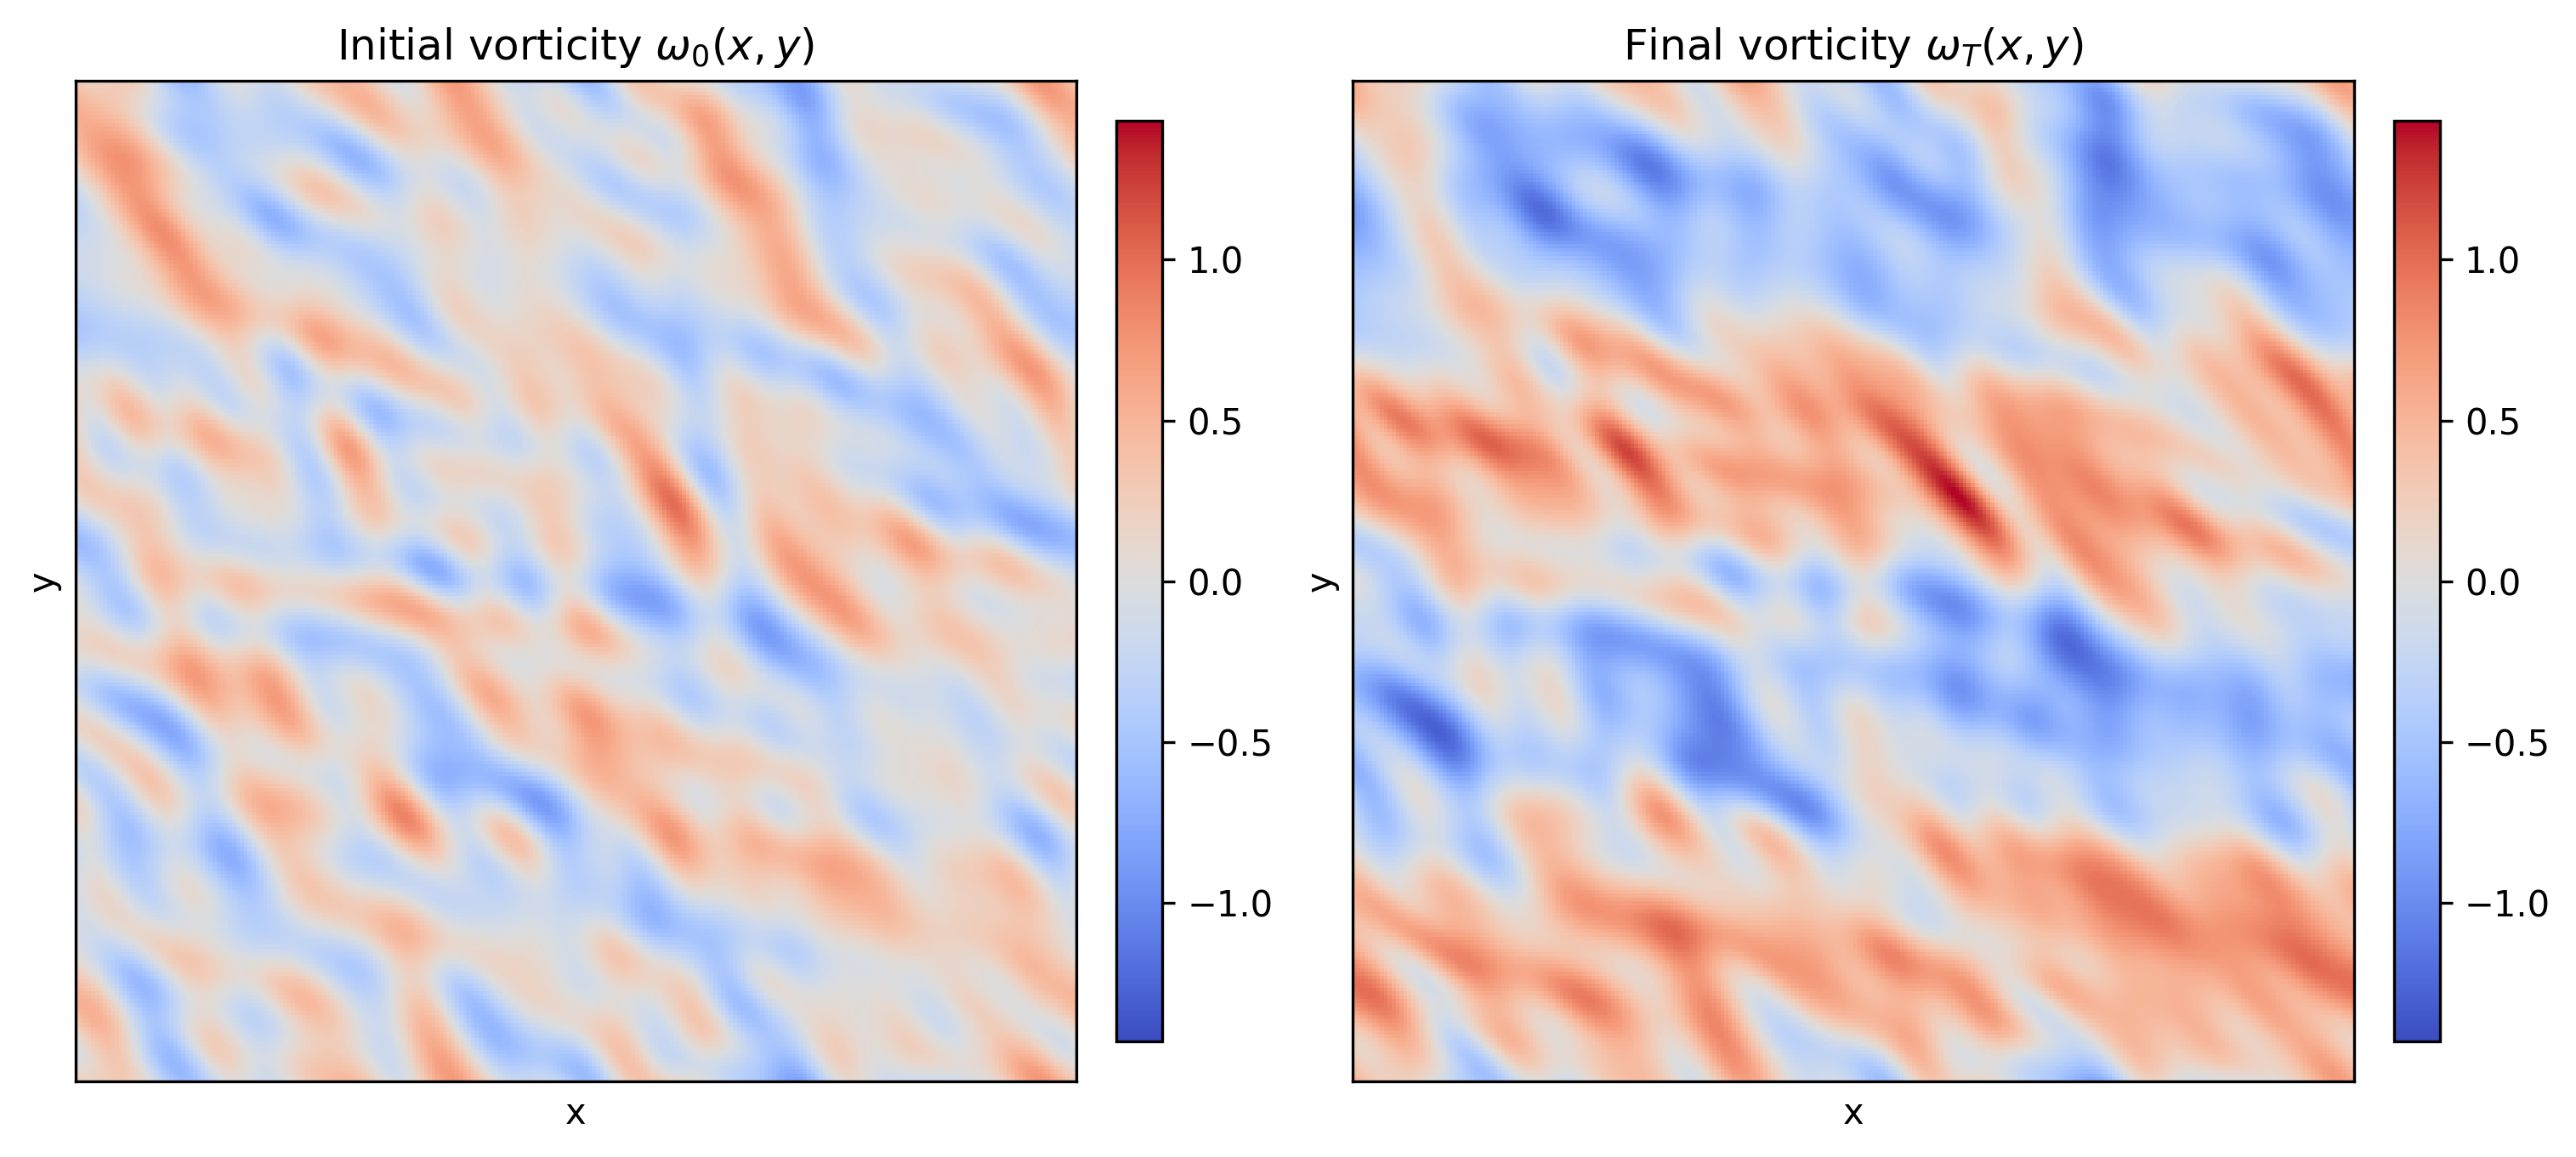
\includegraphics[width=0.8\textwidth]{figures/navier_input_output.png}
    \caption{\label{fig:navier} Initial and final vorticity fields for a sample from the Navier-Stokes dataset.}
\end{figure}

For the regular-grid experiments, we use a two-dimensional Navier-Stokes dataset on the unit square. The Navier-Stokes equations are among the fundamental equations of fluid dynamics and arise in many areas of physics and engineering, including atmospheric and oceanic flows, aerodynamics, and industrial transport processes. The dataset is formulated and solved in vorticity form, with governing equation:


\begin{equation}
    \partial_t \omega + u \cdot \nabla \omega = \nu \Delta \omega + f,
\end{equation}

where $\omega$ denotes the vorticity field, $u$ the incompressible velocity field, $\nu$ the viscosity, and $f$ an external forcing term. The learning task considered in this thesis is not a pressure or velocity prediction problem, but an operator mapping from an initial vorticity field to a later vorticity field. The input to the model is the initial vorticity field $\omega(\cdot,0)$, and the output is the vorticity field at a later time $\omega(\cdot,T)$. An example input-output pair is shown in Figure~\ref{fig:navier}.

The dataset consists of 1000 samples generated at a resolution of $256 \times 256$. Between samples, the viscosity and forcing remain fixed, while the initial vorticity field is varied. Further dataset details and explanation of the data-generation procedure are provided in Appendix~\ref{navier-details}.

\subsubsection{Darcy flow}\label{darcy-flow}

Also used for the uniform-grid experiments is the Darcy flow dataset introduced by Li et al. \cite{li2021fno}. 
In this benchmark, the task is to learn the solution operator of a steady-state two-dimensional Darcy flow problem
on the unit square, governed by the following PDE:

\begin{equation}
    -\nabla \cdot (a(x)\nabla u(x)) = f(x), \qquad x \in (0,1)^2,
\end{equation}
\begin{equation}
    u(x) = 0, \qquad x \in \partial(0,1)^2,
\end{equation}

\begin{figure}
    \centering
    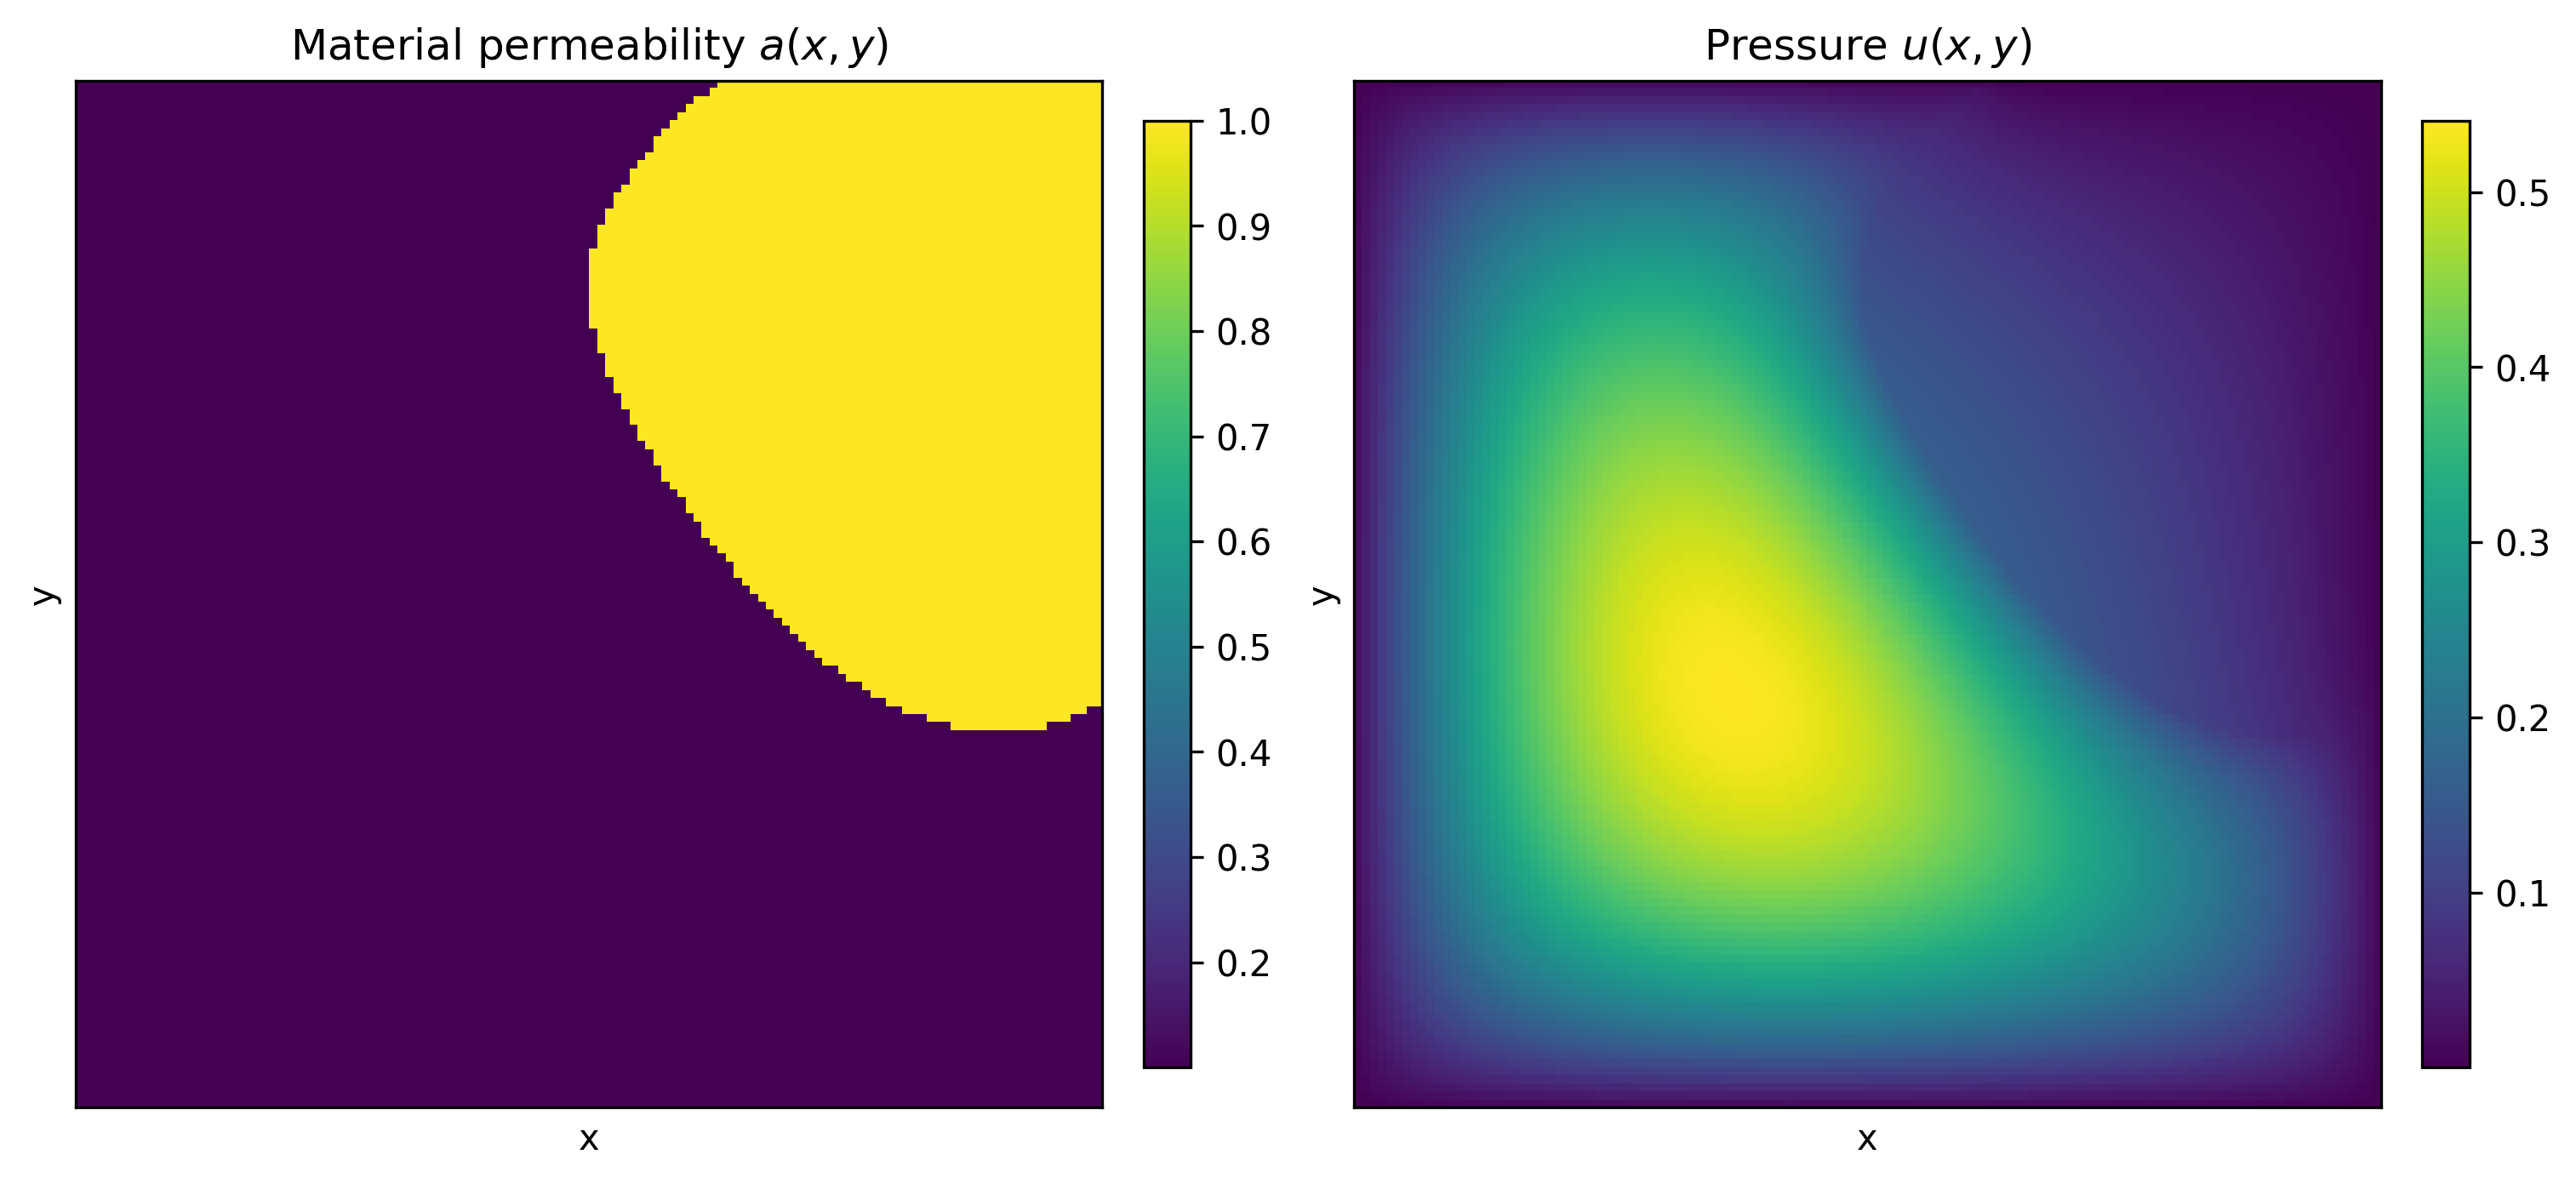
\includegraphics[width=0.9\textwidth]{figures/darcy_input_output.png}
    \caption{\label{fig:darcy} Example of an input diffusion coefficient field \(a(x,y)\) and the resulting pressure
    field \(u(x,y)\) with Dirichlet boundary conditions.}
\end{figure}

The input is a spatially varying permeability field \(a(x)\), and the output is the corresponding pressure field \(u(x)\) under a prescribed forcing term and Dirichlet boundary conditions. An example
 input-output mapping can be seen in figure \ref{fig:darcy}. Between samples, $f(x)$ is kept constant while the $a(x)$ is varied. This PDE has many applications within physics and engineering, including drainage and irrigation in agricultural soils and fluid migration around nuclear waste repositories \cite{darcyapplications}. For this 
  thesis, the Darcy flow dataset serves as a regular-grid benchmark for evaluating the performance of FNO and CNO 
  across discretizations. This dataset was selected because it provides a comparatively smooth benchmark, 
  complementing the more irregular and turbulent behavior of the Navier-Stokes dataset discussed in Section~\ref{navier-stokes}. Using both datasets makes it possible to evaluate model performance under qualitatively different solution regimes. The dataset contains 10000 samples at a resolution of 128$\times$128.



\subsection{Non-Uniform Datasets}\label{non-uniform-datasets}

The experiments on irregular domains primarily use two datasets: an incompressible Navier\hyp{}Stokes
dataset modeling flow past a cylinder and a nuclear engineering
dataset consisting of temperature profiles for a single high temperature gas-cooled reactor (HTGR) column.

\subsubsection{Incompressible Navier-Stokes flow past a cylinder}\label{cylinder-flow-dataset}


The first non-uniform benchmark is an incompressible Navier-Stokes dataset
describing fluid flow past a cylinder. This dataset was used in prior
work on operator learning for PDEs and is included here because it
provides a fluid-dynamics test case on a geometry that is not naturally
aligned with a regular grid \cite{calm-pde, pfaff-datasets}.

The dataset describes two-dimensional incompressible flow with velocity
$\mathbf{v}$ and pressure $p$, governed by:

\begin{equation}
    \nabla \cdot \mathbf{v} = 0,
\end{equation}
\begin{equation}
    \rho_0 \left(\partial_t \mathbf{v} + \mathbf{v} \cdot \nabla \mathbf{v}\right) + \nabla p
    = \mu \nabla^2 \mathbf{v},
\end{equation}

\begin{figure}
    \centering
    \makebox[\textwidth][c]{%
        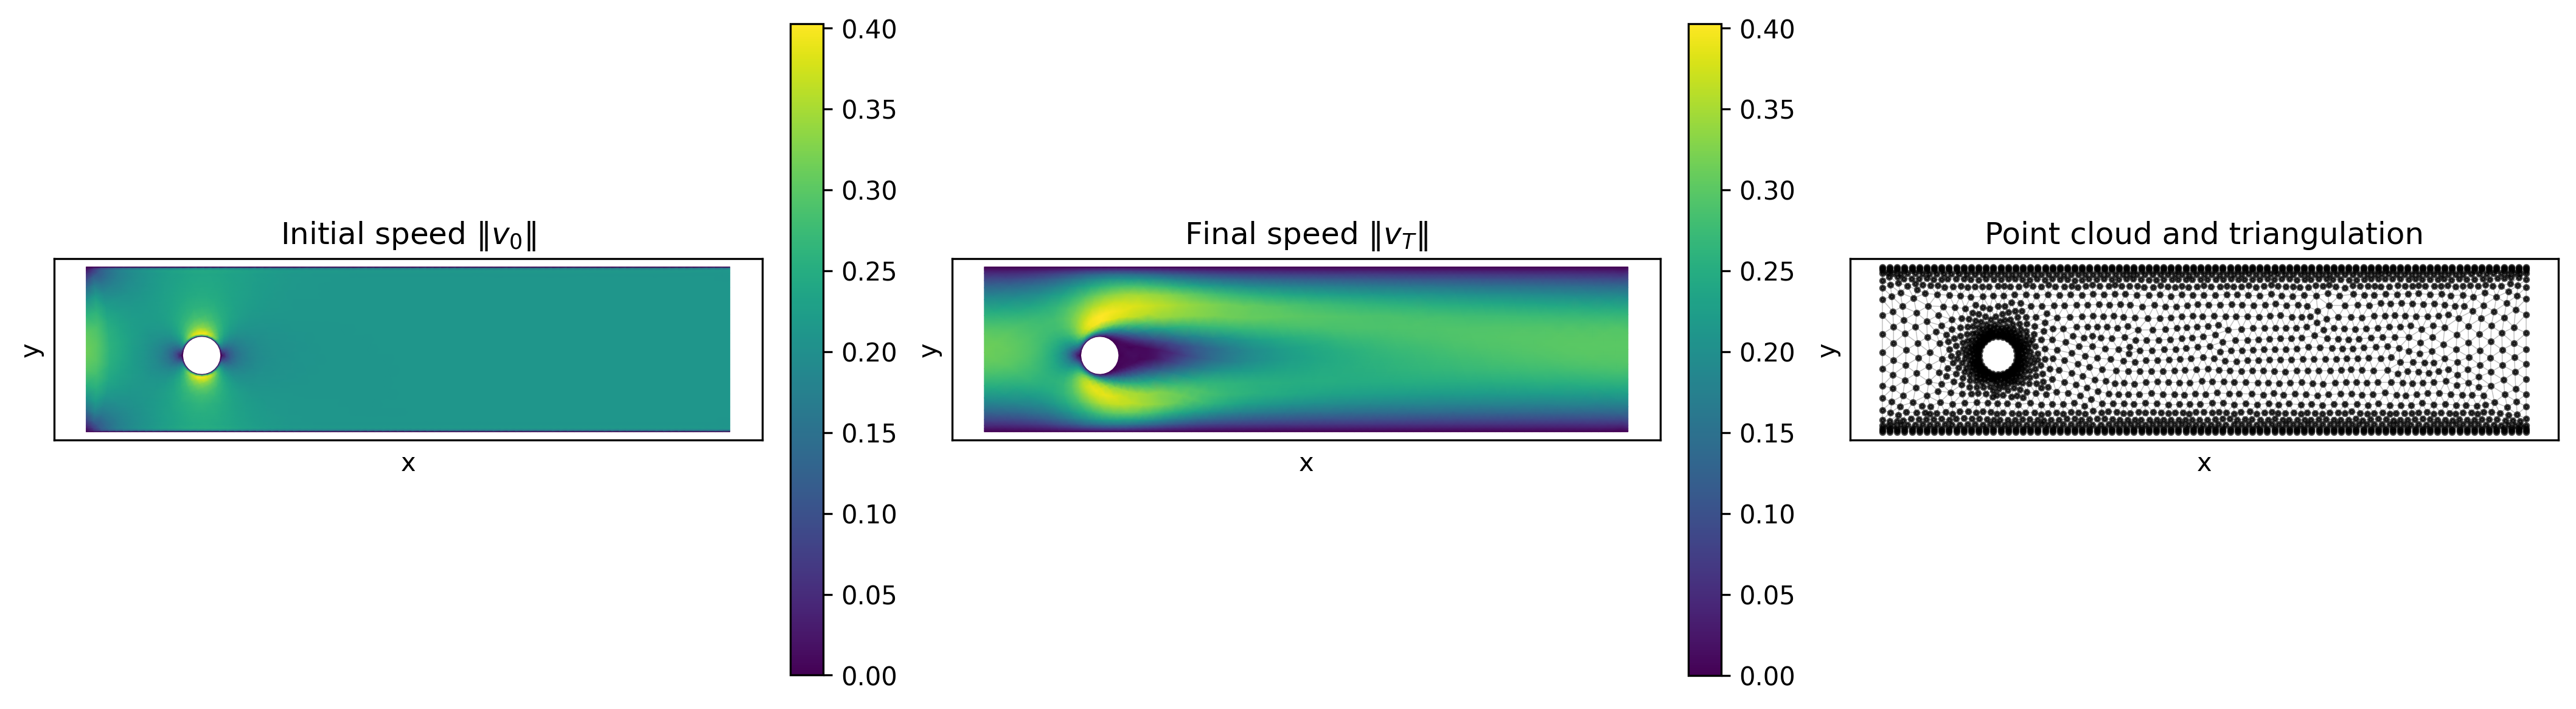
\includegraphics[width=1.1\textwidth]{figures/cylinder_flow_input_output.png}%
    }
    \caption{Example initial and final states
    for the incompressible flow past a cylinder dataset, shown on the
    irregular geometry together with the underlying point cloud. While the model is tasked with predicting the $v_x$ and $v_y$ components of the velocity field, these plots display the speed $\lVert \mathbf{v} \rVert$.}
    \label{fig:cylinder-flow}
\end{figure}

where $\rho_0$ is the constant density and $\mu$ the viscosity. The
domain consists of a channel containing a cylindrical obstacle, with the
cylinder position and radius varying between samples.

The prediction task is to learn a mapping from the initial pressure and velocity fields to the final velocity field, while
accounting for the fact that changes in cylinder size and location lead
to different corresponding flow patterns. In the experiments of this
thesis, the model is trained to predict only the horizontal and vertical
velocity components; pressure is not included in the target.

This dataset is particularly relevant for Geo-FNO because it is defined on a non-uniform spatial discretization rather than a regular Cartesian grid. An example initial-final pair is shown in Figure~\ref{fig:cylinder-flow}. The dataset uses a predefined train-validation-test split, with 1000 training samples, 100 validation samples, and 100 test samples. Each sample contains between 1700 and 2100 points, depending on the geometry of the sample.

\subsubsection{High-Temperature Gas-Cooled Reactor (HTGR) Column Temperature Dataset}\label{htgr-column-dataset}



The next non-uniform dataset consists of steady-state temperature
profiles for a single column of a prismatic core
HTGR. This dataset is included because it provides a first
application-oriented test case for Geo-FNO in a nuclear engineering
setting. Unlike the public benchmark datasets considered earlier, the
data was produced as part of ongoing work by a colleague within the Reactor Physics and Nuclear Materials (RPNM) group of Delft University of Technology.

Physically, the dataset describes the temperature distribution within a
three-dimensional reactor column. For each case, a constant boundary
temperature is imposed and a coupled neutronics-thermohydraulics
calculation is performed until a steady state is reached. The transient
evolution toward this steady state is not included in the dataset; only
the final steady-state temperature fields are used. The use of a fixed
boundary temperature is a simplifying assumption, since in a realistic
reactor system the boundary temperature would itself change as the system
evolves. This simplification was made to produce a controlled dataset
within the time constraints of the project.


The spatial sampling locations lie on an irregular mesh that is shared across all samples. Along the axial direction, the column is quantized into 17 distinct \(z\)-levels. In this thesis, the three-dimensional column data is reformulated as a slice-wise two-dimensional prediction problem: each horizontal slice at a given \(z\)-level is treated as one sample, and the axial coordinate \(z\) is provided as an input parameter to the model. The imposed boundary temperature ranges from \(300\,^{\circ}\mathrm{C}\) to \(1000\,^{\circ}\mathrm{C}\) in steps of \(1\,^{\circ}\mathrm{C}\), yielding 701 distinct thermal conditions. This results in a total of \(17\times701=11917\) two-dimensional samples.

\begin{figure}
    \centering
    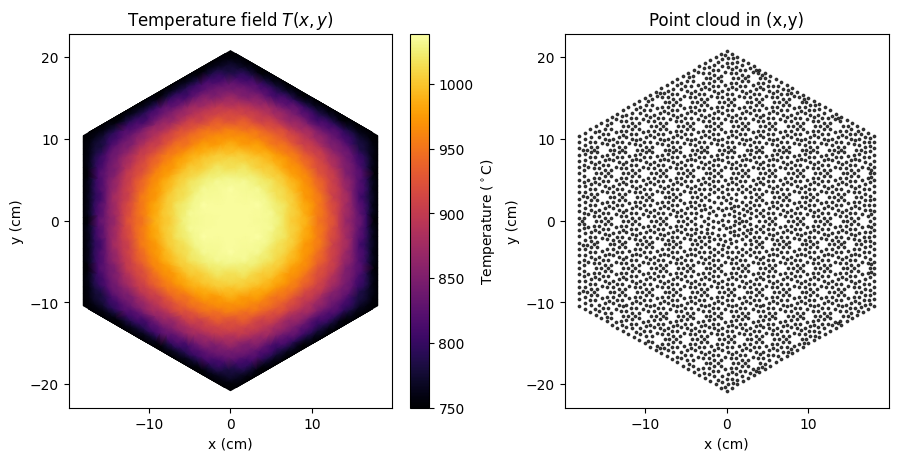
\includegraphics[width=0.8\textwidth]{figures/htgr_column_example.png}
    \caption{\label{fig:htgr-column} Example temperature field from the
    HTGR column dataset for a fixed boundary temperature and selected
    axial layer, shown together with the irregular spatial mesh used for
    sampling. This sample corresponds to an axial level of \(z=30\,\mathrm{cm}\) and a boundary temperature of \(T=750\,^{\circ}\mathrm{C}\).}
\end{figure}

The slices should not be interpreted as independent physical systems. The original temperature fields are generated from a three-dimensional calculation, so axial coupling is already reflected in the resulting temperature profiles. However, the model used in this thesis does not explicitly model interactions between neighboring slices. Instead, it learns a parametric mapping from the imposed boundary temperature and axial coordinate to the temperature distribution on the corresponding horizontal slice.


In the prediction task considered in this thesis, the model receives the
boundary temperature together with a specified $z$-level and predicts
the temperature at all sampled $(x,y)$ locations in the corresponding
horizontal slice. The task can therefore be interpreted as learning a
mapping from the boundary condition and axial position to the
two-dimensional temperature profile within that layer. An example of
such a slice, together with the underlying irregular mesh, is shown in
Figure~\ref{fig:htgr-column}.


\section{Training Setup}

All models are trained in a supervised setting on paired input-output
samples. For each dataset, the available samples were split into training, validation, and test sets. The training set was used to optimize model parameters, while the validation set was used to monitor training and select the final checkpoint. Final reported losses are computed on the test set.

The hyperparameters differ between the uniform-grid and
non-uniform-grid experiments, as well as between datasets. To keep the main text focused on the experimental
design rather than implementation details, hyperparameter settings and training details are given in Appendix~\ref{appendix:hyperparameters}.

Some experiments use feature engineering, meaning that available input variables are transformed before being passed to the model. The purpose is to express the same information in a form that is easier for the network to use, which can improve predictive performance~\cite{feature-engineering}. This is used primarily for the non-uniform datasets, where geometry and low-dimensional parameters play an important role. The specific input representations used for each dataset are described in the corresponding dataset sections.


\section{Uniform-Grid Resolution Transfer Experiments}\label{uniform-experiments}

The uniform-grid experiments are designed to evaluate discretization
invariance by testing how well a model trained at one spatial resolution
generalizes to other resolutions. The Navier-Stokes and Darcy flow
datasets described in \ref{navier-stokes} are used for these experiments. For each dataset, the models are trained at a chosen training resolution and then
evaluated both at the training resolution and at lower and higher
resolutions. This makes it possible to compare performance at the
training resolution with performance after transferring the same trained
model to different spatial resolutions. Both datasets are generated at a single spatial resolution; other resolutions are generated by resampling the data using bicubic interpolation.

For the Navier-Stokes dataset, the models are trained at a resolution of
$192 \times 192$ and evaluated on resolutions from $128 \times 128$ to
$256 \times 256$ in steps of 16 grid points. For the Darcy flow dataset,
the models are trained at a resolution of $96 \times 96$ and evaluated
on resolutions from $64 \times 64$ to $128 \times 128$ in steps of 8
grid points.

Four model variants are compared for each dataset. The first two are FNO
models retaining either 8 or 16 Fourier modes in each spatial direction,
denoted FNO\_k8 and FNO\_k16. The other two are CNO variants. The first is
the regular CNO architecture as outlined in section \ref{sec:cno}, referred to as CNO\_standard. The second is a modified CNO in which the
upsample-nonlinearity-downsample (UND) operation is replaced by a simple pointwise nonlinearity, referred to as CNO\_no\_UND. This operation is one of the architectural changes that distinguishes the CNO from a
U-Net-like architecture and is intended to reduce aliasing effects
introduced by nonlinearities. Comparing the standard and modified CNO
therefore makes it possible to assess the effect of this component in
the resolution-transfer setting.

FNO and CNO handle changes in resolution differently. FNO produces
predictions at the same resolution as the input it is given. In the FNO experiments, evaluation at a resolution \(N \times N\) was performed by first resampling both the input and target fields to \(N \times N\). The resampled input was then passed to the trained FNO, which produces an output on the same grid. This prediction was compared directly with the resampled target field. The CNO, however,
produces predictions on its internal resolution. Therefore, when CNO is
evaluated on an input resolution different from its internal resolution,
the CNO prediction is resampled onto the input resolution before the
error is computed. The target field is resampled to the same resolution,
so that both FNO and CNO are evaluated against target fields on the same
spatial grid. All resampling in these experiments is performed with
bicubic interpolation.





In addition to reporting the mean squared error at each tested resolution, a scalar measure is used to summarize how strongly the loss changes away from the training resolution. Let \(\mathcal{S}\) denote the set of tested resolutions, let \(L_N\) denote the mean squared error at resolution \(N\)\footnote{All uniform-grid experiments in this thesis use square grids. A resolution denoted by \(N\) therefore corresponds to an \(N\times N\) grid, containing \(N^2\) spatial points. This differs from the notation \(n\) used earlier for the total number of grid points.}, and let \(N_{\mathrm{train}}\) denote the training resolution. The discretization variance value is defined as
\begin{equation}
D =
\frac{1}{|\mathcal{S}|}
\sum_{N\in\mathcal{S}}
\left|
\ln(L_N)-\ln(L_{N_{\mathrm{train}}})
\right|.
\end{equation}

The logarithm is used so that the score measures relative, rather than absolute, changes in loss. Equivalently,
\[
\ln(L_N)-\ln(L_{N_{\mathrm{train}}})
=
\ln\left(\frac{L_N}{L_{N_{\mathrm{train}}}}\right),
\]
so \(D\) measures the average multiplicative change in loss relative to the training resolution. For example, a doubling and a halving of the loss contribute equally to \(D\). This makes the score useful for comparing robustness across models whose absolute losses may differ by orders of magnitude.\footnote{In the implementation, a small numerical constant \(\epsilon=10^{-8}\) is added inside the logarithm to avoid numerical issues when losses are very small.}

Lower values of \(D\) indicate that the loss remains closer to the loss at the training resolution across the evaluated resolutions. This score is only a measure of consistency across resolutions, not of absolute model quality. The loss values themselves remain the primary measure of predictive performance, while \(D\) is used only as a quantitative measure of discretization robustness.


\section{Non-Uniform-Grid Geo-FNO Evaluations}\label{non-uniform-experiments}

The non-uniform-grid evaluations use Geo-FNO on the cylinder flow and
HTGR column temperature datasets described in
Section~\ref{non-uniform-datasets}. These evaluations differ from the
uniform-grid resolution transfer experiments in
Section~\ref{uniform-experiments}. Since the spatial samples are given
as point clouds or irregular meshes rather than Cartesian grids, there
is no single resolution parameter equivalent to the grid size $N$ used
in the uniform-grid experiments. The goal is therefore not to measure
resolution transfer, but to evaluate whether Geo-FNO can learn mappings
on irregular spatial data.

For the cylinder flow dataset, the model did not produce meaningful
predictions when it was given only the velocity field on the irregular
mesh. The coordinate transform MLP $\phi^{-1}$ was given the x and y coordinates of the cylinder's center and its radius in the form of the geometric vector $g$. In addition to the horizontal and vertical velocity
components and pressure, each mesh point was also assigned a one-hot encoding of its node
type. The node-type categories distinguish the upper, lower and cylinder boundary nodes, left boundary nodes, right boundary nodes, and interior nodes. This made the location of the obstacle more
explicit in the pointwise input representation, allowing the model to
identify which mesh points lie on or near the cylinder.

For the HTGR column temperature dataset, the raw input consists only of
the boundary temperature $T$ and the axial level $z$. Since this is a
low-dimensional representation of the input conditions, several
alternative representations of $T$ and $z$ were tested through feature engineering. These input
representations and their effect on model performance are discussed in
Appendix~\ref{appendix:htgr-input-engineering}. The best performing representation was used for the results reported in the main text.

Following the discussion in Section~\ref{mesh-free-discretization-invariance}, the non-uniform-grid experiments are treated as held-out evaluations of Geo-FNO on irregular spatial representations. They are not used to compute a mesh-free analogue of the uniform-grid discretization variance value, because the available datasets do not contain controlled refinement families of the same physical samples. The seam artifact observed in early Geo-FNO predictions, and the implementation bug that caused it, are discussed separately in Appendix~\ref{cha:geo-fno-bug-fix}. The results in the main text are reported using the corrected implementation.
\chapter{\label{cha:uniform-results-discussion} Uniform Grids -- Results and Discussion}

\section{Results}

\subsection{Navier-Stokes}




\begin{figure}
    \centering
    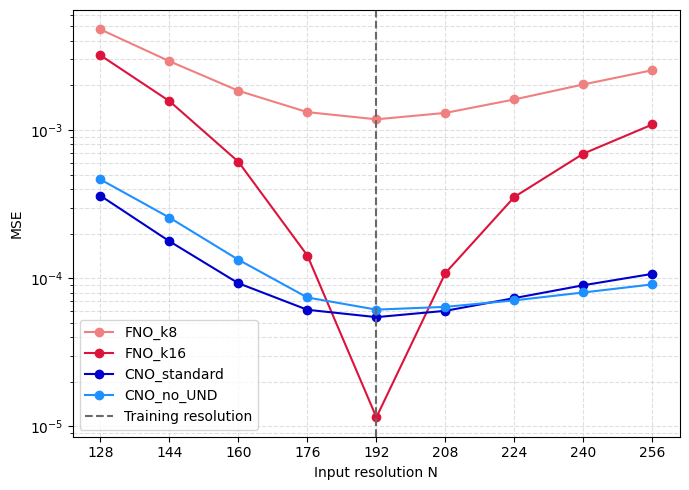
\includegraphics[width=0.8\textwidth]{figures/loss_vs_resolution_navier_stokes.png}
    \caption{\label{fig:loss_vs_resolution_navier_stokes} A plot of the MSE loss as a function of resolution for the four models trained on the Navier-Stokes dataset. The training resolution is indicated by the vertical dashed line.}
\end{figure}

\begin{table}
    \centering
    \caption{\label{tab:d-values-navier-stokes} Discretization variance value $D$ for the Navier-Stokes uniform-grid experiment. Lower values indicate that the loss remains more consistent across evaluation resolutions relative to the loss at the training resolution.}
    \begin{tabular}{lc}
        \hline
        Model & $D$ \\
        \hline
        FNO\_k8 & 0.5076 \\
        FNO\_k16 & 3.4817 \\
        CNO\_standard & 0.5854 \\
        CNO\_no\_UND & 0.5847 \\
        \hline
    \end{tabular}
\end{table}

The four models outlined in Section~\ref{uniform-experiments} were
evaluated on the Navier-Stokes dataset. Figure~\ref{fig:loss_vs_resolution_navier_stokes}
shows the mean squared error (MSE) loss as a function of evaluation resolution for each
model, with the training resolution indicated by the vertical dashed
line. Table~\ref{tab:d-values-navier-stokes} reports the discretization
variance value $D$, which measures how much the loss changes across
resolutions relative to the loss at the training resolution.

Among the FNO models, FNO\_k16 achieves the lowest loss at the training
resolution, but also has the largest value of $D$. Its performance
therefore changes the most under resolution transfer. This contrast is
especially pronounced at the lowest tested resolution, where the loss of
FNO\_k16 increases by more than two orders of magnitude compared with
its loss at the training resolution. FNO\_k8 has a higher loss at all tested resolutions including the training resolution, but a substantially lower value of $D$, indicating
a more consistent loss across the evaluated resolutions. For both FNO
variants, the loss increases more rapidly when evaluating below the
training resolution than when evaluating above it.

The two CNO variants show much flatter loss curves than FNO\_k16 and
have nearly identical values of $D$. Their training-resolution losses are
also comparable. The standard CNO performs slightly better at the
training resolution, at lower resolutions, and at $N = 208$. At the
highest evaluated resolutions, CNO\_no\_UND gives slightly lower losses
than CNO\_standard. Overall, the Navier-Stokes results show a trade-off:
FNO\_k16 gives the best performance at the training resolution, while
FNO\_k8 and the CNO variants show more consistent behavior across
resolutions.



\subsection{Darcy flow}

\begin{figure}
    \centering
    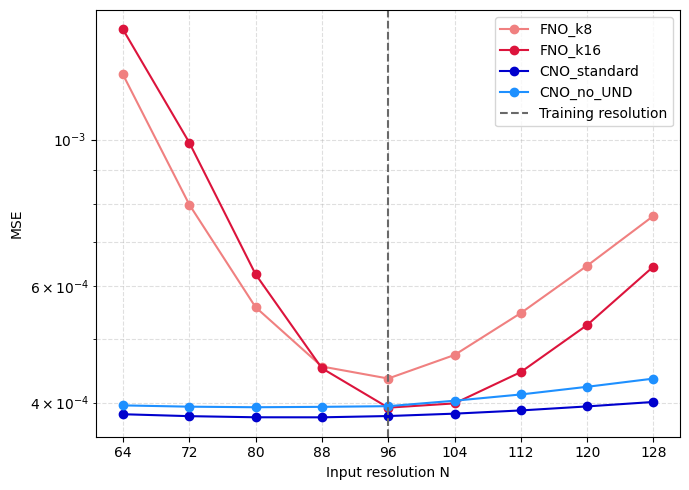
\includegraphics[width=0.8\textwidth]{figures/loss_vs_resolution_darcy_flow.png}
    \caption{\label{fig:loss_vs_resolution_darcy_flow} A plot of the MSE loss as a function of resolution for the four models trained on the Darcy flow dataset. The training resolution is indicated by the vertical dashed line.}
\end{figure}


To test whether the trends observed on the Navier-Stokes dataset also
appear on a qualitatively different PDE benchmark, the four models were
evaluated on the Darcy flow dataset. The Darcy flow dataset was chosen as the solution space is smooth, making it a good point of comparison to the Navier-Stokes dataset. Figure~\ref{fig:loss_vs_resolution_darcy_flow}
shows the MSE loss as a function of evaluation resolution for each
model, with the training resolution indicated by the vertical dashed
line. Table~\ref{tab:d-values-darcy-flow} reports the corresponding
discretization variance value $D$.

\begin{table}
    \centering
    \caption{\label{tab:d-values-darcy-flow} Discretization variance value $D$ for the Darcy flow uniform-grid experiment. Lower values indicate that the loss remains more consistent across evaluation resolutions relative to the loss at the training resolution.}
    \begin{tabular}{lc}
        \hline
        Model & $D$ \\
        \hline
        FNO\_k8 & 0.3583 \\
        FNO\_k16 & 0.4179 \\
        CNO\_standard & 0.0140 \\
        CNO\_no\_UND & 0.0260 \\
        \hline
    \end{tabular}
\end{table}

Compared with the Navier-Stokes experiment, the four models are closer
in overall performance on the Darcy flow dataset. At the training
resolution, CNO\_standard achieves the lowest loss, followed by
FNO\_k16, CNO\_no\_UND, and FNO\_k8. The two FNO variants show a similar
pattern to that observed for Navier-Stokes; the loss is lowest near the
training resolution and increases when the model is evaluated at other
resolutions. This increase is stronger below the training resolution
than above it. Notably, FNO\_k8 outperforms FNO\_k16 at resolutions below $N = 88$. This indicates that
retaining more Fourier modes does not consistently improve performance
under transfer to coarser grids.

The CNO variants show much flatter loss curves across the evaluated
resolutions, with $D$ values of order \(10^{-2}\). At lower resolutions,
both CNO models maintain an almost constant loss, while at higher
resolutions both losses increase slowly. In contrast to the
Navier-Stokes experiment, CNO\_standard outperforms CNO\_no\_UND at all
evaluated resolutions. The loss of CNO\_no\_UND also increases more
quickly than that of CNO\_standard when evaluating above the training
resolution. Overall, the Darcy flow results show a clearer separation
between the FNO and CNO variants in terms of discretization robustness;
the FNO models are more sensitive to resolution transfer, while the CNO
models remain nearly constant across the tested range.


\subsubsection{FNO resolution-transfer diagnostics}\label{sec:fno_diagnostics}

The results in Figures~\ref{fig:loss_vs_resolution_navier_stokes} and~\ref{fig:loss_vs_resolution_darcy_flow} show that the FNO variants are more sensitive to changes in evaluation resolution than the CNO variants. This effect is most pronounced for FNO\_k16 on the Navier--Stokes dataset, which achieves a low loss at the training resolution but a substantially higher loss away from it. To investigate this behavior in more detail, three additional diagnostics were performed using FNO\_k16 on the Navier--Stokes dataset. These diagnostics were evaluated at the lowest tested resolution \(N=128\), the training resolution \(N=192\), and the highest tested resolution \(N=256\).

\begin{figure}
    \centering
    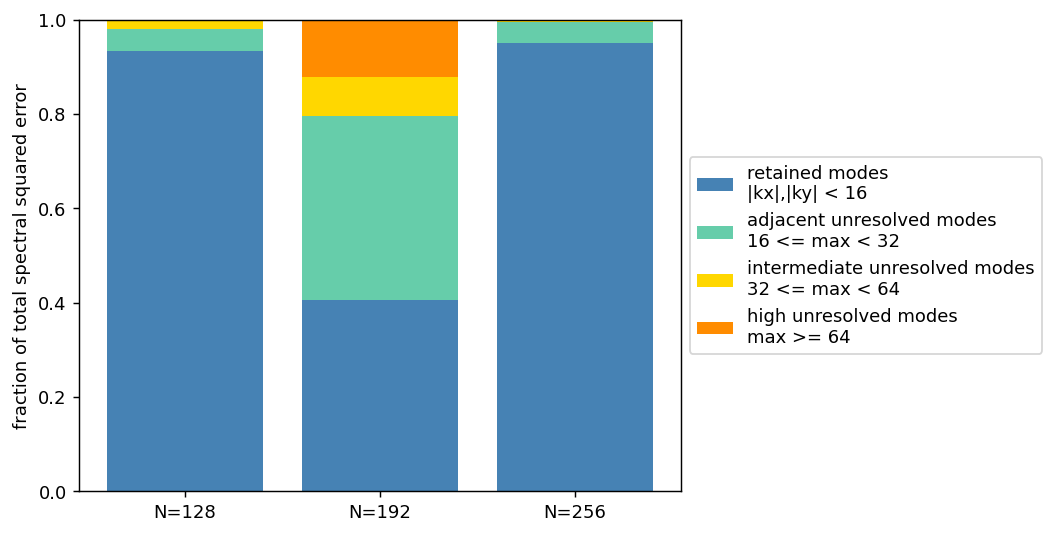
\includegraphics[width=0.85\textwidth]{figures/fno_error_bands.png}
    \caption{Fraction of total spectral squared error by Fourier box band for FNO k16 on the Navier--Stokes dataset. Here max denotes \(max(|k_x|,|k_y|)\). The first band, \(|k_x|,|k_y|<16\), corresponds to the modes retained by the FNO\_k16 spectral convolution.}
    \label{fig:fno_error_bands}
\end{figure}

First, the prediction error was decomposed in Fourier space. For each of the three resolutions, the pointwise difference between the model prediction and the ground truth was computed and transformed into Fourier space. The squared magnitudes of the resulting Fourier coefficients were then grouped into bands. The first band, \(|k_x|,|k_y|<16\), corresponds to the Fourier modes retained by the FNO k16 model. Figure~\ref{fig:fno_error_bands} shows the fraction of total spectral squared error in each band for \(N=128\), \(N=192\), and \(N=256\).

At the training resolution \(N=192\), the error is distributed across several spectral bands. The retained modes account for approximately \(40.6\%\) of the total spectral error, while the adjacent unresolved modes account for approximately \(39.1\%\). At the transfer resolutions, the distribution changes substantially: the retained modes account for approximately \(93.3\%\) of the error at \(N=128\) and \(95.1\%\) at \(N=256\). Since the overall prediction error is much larger at these transfer resolutions, this indicates that the increased error is concentrated primarily in the modes explicitly retained by the FNO, rather than only in modes outside the spectral cutoff.

This diagnostic localizes the error, but does not by itself identify its cause. The following diagnostics therefore test whether this retained-mode error comes from changes in the represented input and target spectra, or from changes introduced during the FNO forward pass.

Second, a spectral-resampling control experiment was performed to separate changes in represented spectral content from changes in spatial evaluation resolution. In the original resolution transfer experiment, fields at different resolutions were obtained using bicubic interpolation. This can slightly change the retained Fourier coefficients of the input and target fields, which makes it difficult to determine whether the observed prediction drift is caused by changes in the represented data or by evaluating the FNO on a different grid.

To test this, the experiment was repeated using spectral resampling. Starting from the \(N=192\) input and target fields, new \(N=128\) and \(N=256\) versions were constructed directly in Fourier space. This produces different grid representations of the same spectrally defined fields. The FNO was then evaluated on both the bicubic-resampled and spectrally resampled fields.

To quantify how much the retained spectral content changes, the retained Fourier coefficients of the input, target, and prediction were compared to their corresponding \(N=192\) coefficients. Because fields at different spatial resolutions have different numbers of grid points, they cannot be compared directly pointwise. The retained Fourier coefficients provide a common representation for the modes shared across resolutions. The following drift measure is therefore used only as a diagnostic for comparing these shared retained modes, not as a general prediction-error metric. For a field \(v\), this drift is defined as
\begin{equation}
\delta_{\mathrm{ret}}(v;N)
=
\frac{
\left\|\hat v_{\mathrm{ret}}^{N}-\hat v_{\mathrm{ret}}^{192}\right\|_2
}{
\left\|\hat v_{\mathrm{ret}}^{192}\right\|_2
},
\label{eq:retained-mode-drift}
\end{equation}
where \(\hat v_{\mathrm{ret}}^{N}\) denotes the vector of retained Fourier coefficients at resolution \(N\), corresponding to \(|k_x|,|k_y|<16\). Table~\ref{tab:fno_spectral_resampling} reports \(\delta_{\mathrm{ret}}\) for the input, target, and prediction, together with the relative \(L^2\) prediction error.

\begin{table}
\centering
\begin{tabular}{llcccc}
\toprule
Resampling & \(N\) & Input drift & Target drift & Prediction drift & Rel. \(L^2\) error \\
\midrule
Bicubic & 128 & \(8.05\times10^{-2}\) & \(4.05\times10^{-2}\) & \(1.24\times10^{-1}\) & \(1.12\times10^{-1}\) \\
Bicubic & 192 & \(0\)                 & \(0\)                 & \(0\)                 & \(2.49\times10^{-3}\) \\
Bicubic & 256 & \(4.03\times10^{-2}\) & \(2.03\times10^{-2}\) & \(7.25\times10^{-2}\) & \(6.67\times10^{-2}\) \\
\midrule
Spectral & 128 & \(1.18\times10^{-7}\) & \(9.82\times10^{-8}\) & \(1.17\times10^{-1}\) & \(1.26\times10^{-1}\) \\
Spectral & 192 & \(0\)                 & \(0\)                 & \(0\)                 & \(7.64\times10^{-3}\) \\
Spectral & 256 & \(1.15\times10^{-7}\) & \(6.38\times10^{-8}\) & \(6.93\times10^{-2}\) & \(6.67\times10^{-2}\) \\
\bottomrule
\end{tabular}
\caption{Comparison of bicubic and spectral resampling for FNO k16 on the Navier--Stokes dataset. Drift is measured in the retained Fourier modes \(|k_x|,|k_y|<16\) relative to the corresponding \(N=192\) coefficients. The spectral resampling experiment removes retained-mode drift in the input and target up to numerical precision, while the prediction drift and relative error remain large.}
\label{tab:fno_spectral_resampling}
\end{table}

With bicubic interpolation, the retained input and target modes already differ from the \(N=192\) representation. At \(N=128\), the input drift is approximately \(8.05\times10^{-2}\), while the target drift is approximately \(4.05\times10^{-2}\). Spectral resampling removes this difference almost entirely, reducing both input and target drift to values of order \(10^{-7}\). However, the prediction drift remains of the same order as in the bicubic case: approximately \(1.17\times10^{-1}\) at \(N=128\) and \(6.93\times10^{-2}\) at \(N=256\). The relative prediction error also remains much larger than at the training resolution. This shows that matching the retained input and target modes is not sufficient to recover the training-resolution behavior. Even when the low-mode content seen by the FNO is held fixed up to numerical precision, the model still produces a different prediction when executed on a different spatial grid. The remaining mismatch must therefore be introduced during the FNO forward pass itself.

Finally, the internal representations of the FNO were compared across spatial resolutions during the forward pass. This diagnostic uses the \(N=192\) forward pass as the reference and applies the retained-mode drift from Equation~\eqref{eq:retained-mode-drift} to each saved intermediate representation. The purpose is to identify where the \(N=128\) and \(N=256\) forward passes first diverge from the training-resolution computation. For readability, Figure~\ref{fig:fno_internal_drift} shows a representative subset of these stages: the model input, lifted representation, padded representation, output after the first activation, and final prediction.

The model input already contains a small amount of drift, while the lifted representation remains at the same order of magnitude. A much larger increase occurs after the spatial padding operation. For \(N=128\), the drift increases from \(7.83\times10^{-3}\) in the lifted representation to \(2.33\times10^{-1}\) after padding; for \(N=256\), it increases from \(3.89\times10^{-3}\) to \(1.28\times10^{-1}\). The drift increases further after the first activation and then remains elevated through the final prediction. This indicates that the representations are still relatively close before padding, but diverge substantially once the padded representation is formed, identifying fixed-cell padding as the main source of resolution-dependent internal drift in this diagnostic.

\begin{figure}
    \centering
    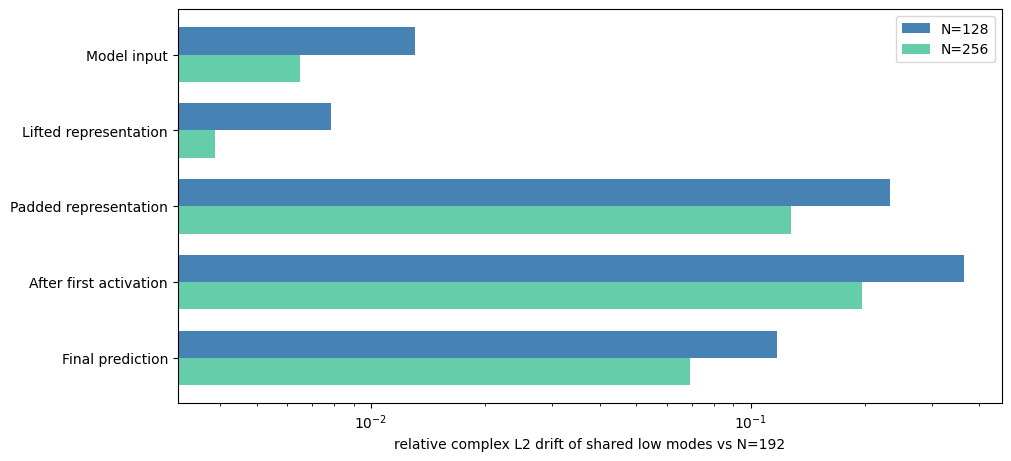
\includegraphics[width=0.9\textwidth]{figures/fno_internal_drift.png}
    \caption{Internal retained-mode drift of FNO k16 relative to the \(N=192\) forward pass. The inputs are spectrally resampled from the \(N=192\) fields. Drift is shown for selected stages of the model, with the largest increase occurring after spatial padding.}
    \label{fig:fno_internal_drift}
\end{figure}

Together, the FNO diagnostics give the following interpretation:
\begin{itemize}
    \item The loss increase at transfer resolutions is not explained simply by high-frequency target content outside the FNO cutoff, since most of the spectral error lies in the retained modes.
    \item Matching the retained input and target modes by spectral resampling does not recover the training-resolution behavior, showing that the mismatch is grid-dependent and introduced during the model forward pass.
    \item The largest layerwise increase in retained-mode drift occurs after spatial padding, identifying fixed-cell padding as the main source of resolution-dependent internal drift in the tested FNO.
\end{itemize}






\subsubsection{CNO high-resolution diagnostics}
\label{sec:cno_diagnostics}

The Navier--Stokes resolution-transfer results show that CNO\_standard and CNO\_no\_UND behave similarly over most of the evaluated range, but CNO\_no\_UND gives slightly lower loss at resolutions above the training resolution. This differs from the Darcy flow results, where CNO\_standard performs better at all evaluated resolutions. Since the only architectural difference between the two CNO variants is the upsample--nonlinearity--downsample block, additional diagnostics were performed to investigate this high-resolution Navier--Stokes behavior.

First, the filtering effect of the UND operation was measured directly. Individual Fourier modes were passed through the upsample--downsample part of the UND block, and the amplitude of the same mode after filtering was compared with its original amplitude. Figure~\ref{fig:cno_und_gain} shows the resulting same-mode gain \(G(k_x,k_y)\) at internal resolution \(N=192\). Values close to one indicate that the filter barely attenuates the mode, while lower values indicate stronger attenuation.

At the finest internal resolution, the UND operation is nearly identity on the lowest modes. In particular, the region where \(G(k_x,k_y)\approx1\) contains the modes used to generate the Navier--Stokes initial conditions. The gain then decreases smoothly toward higher wavenumbers, showing that the UND filter acts as a gradual low-pass operation rather than a sharp spectral cutoff.

The gain pattern should be interpreted relative to the bandwidth of the grid on which the UND operation is applied. At \(N=192\), the plotted quadrant extends to the Nyquist mode \(96\); if the spatial resolution is halved to \(N=96\), the same pattern extends only to mode \(48\). Thus, as the CNO encoder downsamples the feature maps, the same physical spatial variation occupies a larger fraction of the available bandwidth and can be more strongly affected by UND filtering in deeper layers.

\begin{figure}
    \centering
    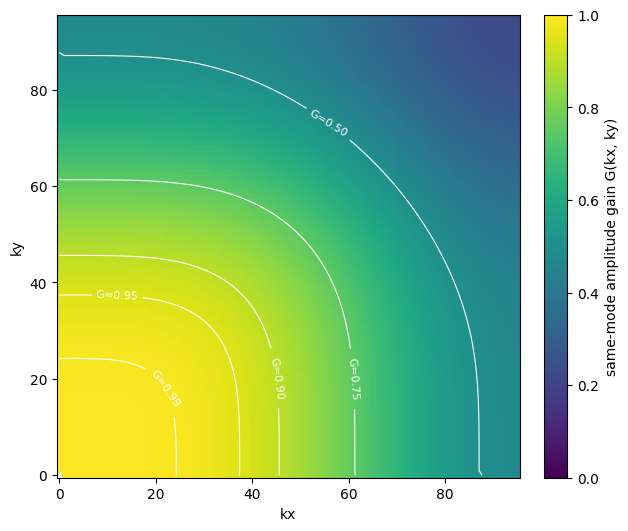
\includegraphics[width=0.85\textwidth]{figures/cno_und_gain.png}
    \caption{\label{fig:cno_und_gain}
    Same-mode amplitude gain \(G(k_x,k_y)\) of the standard UND upsample--downsample filtering operation at internal resolution \(N=192\). Values near one indicate that the filter has little effect on that mode, while lower values indicate stronger attenuation. The response is nearly identity for low modes and decreases smoothly toward higher wavenumbers.}
\end{figure}

Second, the prediction error of CNO\_standard and CNO\_no\_UND was decomposed by Fourier band at \(N=256\). Because CNO predictions are produced on the fixed internal grid before being resampled to the requested evaluation resolution, a comparison performed only after interpolation to \(N=256\) could mix model error with interpolation effects. To avoid this, the raw \(192\times192\) CNO outputs were compared with the \(N=256\) target projected to the same \(192\times192\) grid. This measures the quality of the native internal output representation before the final interpolation step.

On this raw output grid, CNO\_no\_UND obtains lower MSE than CNO\_standard:
\[
\mathrm{MSE}_{\mathrm{standard}} = 1.02\times 10^{-4},
\qquad
\mathrm{MSE}_{\mathrm{no\_UND}} = 8.54\times 10^{-5}.
\]
Figure~\ref{fig:cno_band_error_raw} shows the ratio between the bandwise spectral errors of the two models. For each Fourier band \(B\), the plotted value is
\[
\frac{E_B^{\mathrm{no\_UND}}}{E_B^{\mathrm{standard}}},
\qquad
E_B=\sum_{k\in B}|\hat u_{\mathrm{pred}}(k)-\hat u_{\mathrm{target}}(k)|^2,
\]
averaged over the test samples. Values below one therefore indicate bands where CNO\_no\_UND has lower error, while values above one indicate bands where CNO\_standard has lower error.

\begin{figure}
    \centering
    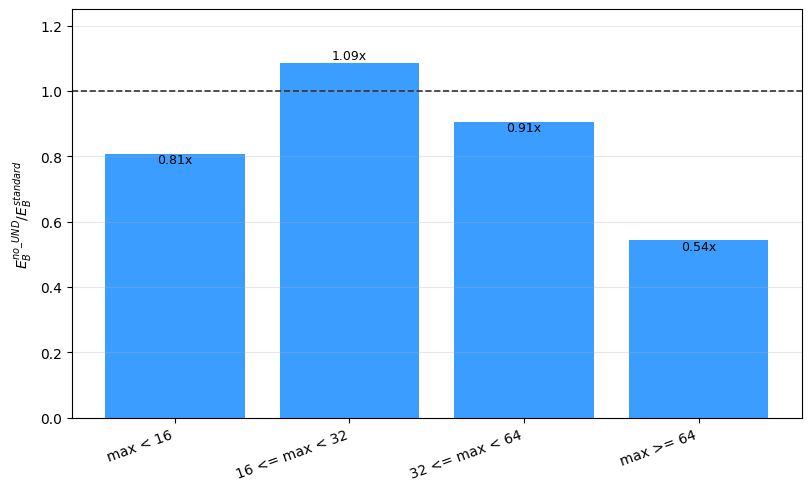
\includegraphics[width=0.8\textwidth]{figures/cno_band_error_raw_grid.png}
    \caption{\label{fig:cno_band_error_raw}
Ratio of box-band spectral error for CNO\_no\_UND relative to CNO\_standard on the raw \(192\times192\) output grid for inputs evaluated at \(N=256\). The \(N=256\) target is projected to the same \(192\times192\) grid before comparison. Here \(max\) is used as shorthand for \(\max(|k_x|,|k_y|)\), so the first band, \(max<16\), contains the modes used to generate the Navier--Stokes initial conditions. For each band \(B\), the plotted value is \(\frac{E_B^{\mathrm{no\_UND}}}{E_B^{\mathrm{standard}}}\), where \(E_B\) is the summed squared Fourier-coefficient error in that band, averaged over the test samples. The dashed line marks equal error. Values below one mean that CNO\_no\_UND has lower error; for example, \(0.81\times\) means that CNO\_no\_UND has \(81\%\) of the CNO\_standard error in that band, corresponding to a \(19\%\) reduction.}
\end{figure}

CNO\_no\_UND has lower error in the lowest band, where \(max<16\), with approximately \(81\%\) of the CNO\_standard error. It is slightly worse in the adjacent band, where \(16\leq max<32\), with approximately \(1.09\) times the CNO\_standard error, and has lower error again in the two higher bands. Since the comparison is performed on the raw \(192\times192\) output grid, this difference is already present before the final interpolation to \(N=256\).

Finally, spatial error maps were computed over the full Navier--Stokes test set at \(N=256\). Figure~\ref{fig:cno_spatial_error_maps} shows the mean squared-error maps for both CNO variants and their difference. Both models exhibit elevated error near the domain boundaries, indicating that these regions are difficult for both architectures. The difference map shows mixed behavior near the boundaries, with regions where CNO\_no\_UND improves and regions where it worsens. In the interior, the difference is smaller and more diffuse, indicating that the improvement is not localized to a single spatial structure.

\begin{figure}
    \centering
    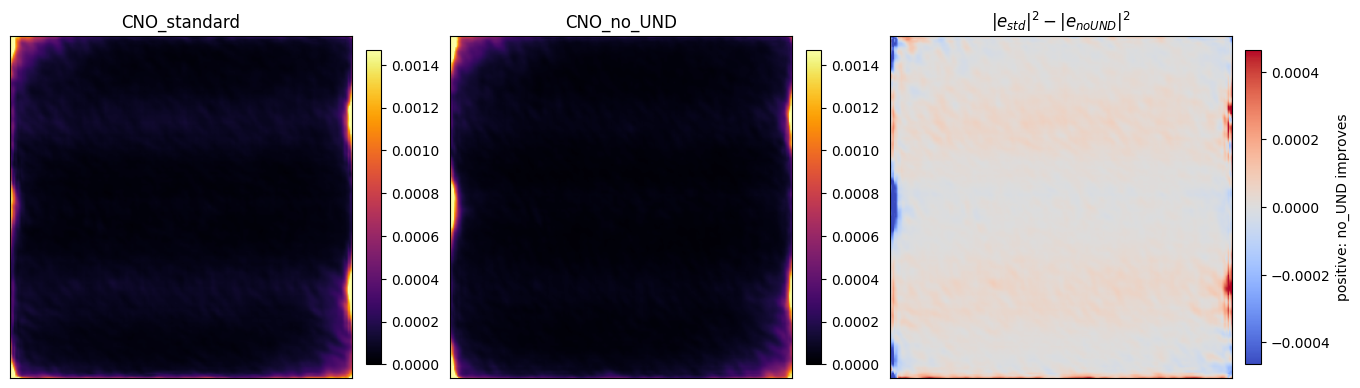
\includegraphics[width=0.95\textwidth]{figures/cno_spatial_error_maps.png}
    \caption{\label{fig:cno_spatial_error_maps}
    Mean spatial squared-error maps over the full Navier--Stokes test set at \(N=256\). The first two panels show the mean squared error for CNO\_standard and CNO\_no\_UND. The third panel shows the difference \(|e_{\mathrm{standard}}|^2-|e_{\mathrm{no\_UND}}|^2\), where positive values indicate regions where CNO\_no\_UND has lower error.}
\end{figure}

Together, the CNO diagnostics give the following interpretation:
\begin{itemize}
    \item The UND upsample--downsample operation acts as a gradual low-pass filter. At the finest internal resolution it barely attenuates the lowest Navier--Stokes modes, but the same filtering pattern becomes more restrictive at coarser internal resolutions where the available bandwidth is smaller.
    \item The high-resolution advantage of CNO\_no\_UND is already present on the raw \(192\times192\) output grid, so it is not primarily caused by the final interpolation to \(N=256\).
    \item The improvement is not only a high-frequency effect. CNO\_no\_UND has its largest practically important reduction in the lowest box band, indicating that removing UND changes the learned representation more broadly.
    \item The spatial error maps do not identify a single localized structure responsible for the improvement. The difference is distributed across the field, with mixed behavior near the boundaries.
\end{itemize}





\section{Discussion}

\subsection{FNO}\label{sec:fno_discussion}

The FNO variants show the weakest discretization robustness of the models tested on both datasets. This is most clearly visible in Figures~\ref{fig:loss_vs_resolution_navier_stokes} and~\ref{fig:loss_vs_resolution_darcy_flow}, where both FNO models show stronger dependence on evaluation resolution than the corresponding CNO models. The effect is particularly pronounced for FNO\_k16 on the Navier--Stokes dataset; FNO\_k16 achieves the lowest loss at the training resolution, but also has the largest value of \(D\) by a large margin. This shows that strong performance at the training resolution does not by itself imply robustness under resolution transfer.

The diagnostic experiments in Section~\ref{sec:fno_diagnostics} indicate that the behavior under resolution transfer is not primarily caused by the FNO simply discarding high-frequency target information. In Figure~\ref{fig:fno_error_bands}, the prediction error at the transfer resolutions is concentrated mainly in the modes explicitly retained by the FNO. At \(N=128\) and \(N=256\), the retained modes account for approximately \(93.3\%\) and \(95.1\%\) of the total spectral error, respectively. If the main issue were only that the target contained unresolved modes outside the spectral cutoff, the dominant error would instead be expected outside the retained band. The observed error distribution therefore points to a failure in the modes that the model is designed to represent directly. 

The spectral-resampling experiment in Table~\ref{tab:fno_spectral_resampling} further separates changes in the represented data from changes in model execution. With bicubic interpolation, the retained input and target modes differ from the \(N=192\) representation, especially at \(N=128\). However, when the \(N=128\) and \(N=256\) fields are constructed by spectral resampling from the \(N=192\) fields, the retained input and target drift is reduced to numerical precision. Despite this, the prediction drift remains large; approximately \(1.17\times10^{-1}\) at \(N=128\) and \(6.93\times10^{-2}\) at \(N=256\). This shows that the poor resolution transfer behavior is not explained simply by the retained Fourier coefficients of the input and target changing across spatial resolutions. Even when these retained coefficients are matched to numerical precision, the FNO still produces a substantially different prediction away from the training resolution. The remaining mismatch must therefore be introduced during the FNO forward pass itself.


The layerwise diagnostic in Figure~\ref{fig:fno_internal_drift} identifies where this resolution dependence enters the model. The model input already contains a small amount of drift relative to the \(N=192\) forward pass. The lifted representation remains at the same order of magnitude, indicating that the lifting layer does not substantially amplify this mismatch.

A much larger increase occurs after the spatial padding operation. For \(N=128\), the retained-mode drift increases from \(7.83\times10^{-3}\) in the lifted representation to \(2.33\times10^{-1}\) after padding. For \(N=256\), it increases from \(3.89\times10^{-3}\) to \(1.28\times10^{-1}\). The drift increases further after the first activation and remains elevated through the final prediction. This shows that the representations are still relatively close before padding, but diverge substantially once the padded representation is formed.

This points to fixed-cell spatial padding as the main implementation-level source of resolution dependence in the tested FNO. Because the FNO uses FFTs, the field passed to each spectral layer is implicitly treated as periodic. For non-periodic data, this creates an artificial discontinuity at the boundary of the periodic extension. Such discontinuities require many Fourier modes to represent and, after spectral truncation, can lead to ringing artifacts near the boundary.

To reduce this effect, the implementation applies zero padding in physical space before the Fourier layers. The Fourier operations are then applied on the enlarged padded domain, but only the original physical region is kept afterward. The padded region therefore acts as a buffer where boundary artifacts from the periodic extension can be absorbed without being directly penalized in the final loss. Equivalently, the model is not forced to make the two opposite edges of the physical domain match each other as they would in a strictly periodic representation.

However, the padding width in the original FNO implementation is specified as a fixed number of grid cells. If \(p\) cells are added to a grid of size \(N\), the physical width of the padded region scales like \(p/N\). Thus, the same padding value corresponds to different physical extensions at \(N=128\), \(N=192\), and \(N=256\). The Fourier transform inside the model is therefore applied to a resolution-dependent padded field rather than to the same physical field represented at different resolutions.

The consequence is that the Fourier transform inside the model is not applied to the same physical field represented at different resolutions. It is applied to different padded extensions of that field. Even if the unpadded input spectrum is held fixed, as in the spectral-resampling experiment, the object passed to the Fourier layers changes once padding is applied. This explains why the prediction still drifts when the retained input and target modes are matched to numerical precision. The learned spectral weights are being applied to internal representations that are no longer resolution-consistent.

This mechanism also explains why the FNO degrades both below and above the training resolution. In both cases, the physical width of the padded region differs from the one used during training. The degradation is stronger below the training resolution, which is likely compounded by the fact that coarser grids are more vulnerable to interpolation error, under-resolution, and possible aliasing. This is reflected in Table~\ref{tab:fno_spectral_resampling}, where bicubic interpolation produces a larger retained-mode input drift at \(N=128\) than at \(N=256\). These effects may contribute to the asymmetry of the loss curve, but they do not explain the main failure by themselves, since spectral resampling removes the input and target drift while the prediction drift remains large.

The particularly sharp minimum of FNO\_k16 on the Navier--Stokes dataset can therefore be understood as a combination of strong training-resolution accuracy and sensitivity to the exact discretization used during training. As described in Appendix~\ref{navier-details}, the initial vorticity fields are generated spectrally using modes with \(0<k_x,k_y<16\) in the positive quadrant, together with the corresponding conjugate modes needed to obtain real-valued fields. An FNO retaining 16 modes is therefore able to represent all Fourier modes present in the initial condition within its spectral layers. This does not mean that the final vorticity field is bandlimited to 16 modes, since the Navier--Stokes dynamics are nonlinear and generate additional higher-frequency content during time evolution. However, it does make FNO\_k16 especially well matched to the input representation at the training resolution, allowing it to achieve a very low loss at \(N=192\). When the same model is evaluated at another resolution, the internal representation changes through the coordinate grid and fixed-cell padding, producing the sharp increase in loss away from the training resolution observed in Figure~\ref{fig:loss_vs_resolution_navier_stokes}.

The comparison between FNO\_k8 and FNO\_k16 should be interpreted in this context. FNO\_k16 can treat all Fourier modes present in the initial Navier--Stokes condition explicitly through its spectral layers. It can therefore rely heavily on the retained Fourier coefficients when learning the mapping at the training resolution. This helps explain its very low loss at \(N=192\), but also makes the model sensitive when those internal coefficients change under resolution transfer. FNO\_k8, by contrast, retains only part of the Fourier content present in the initial condition. A larger fraction of the mapping must therefore be represented indirectly through the pointwise channel mixing and nonlinearities. This makes FNO\_k8 less accurate, but also less dependent on the full retained spectral representation being exactly the same as during training. As a result, FNO\_k8 shows a much lower value of \(D\), while FNO\_k16 gives better absolute accuracy but is more strongly tied to the training-resolution computation.

On the Darcy flow dataset, the same qualitative behavior appears but is less extreme. The Darcy input fields are not constructed to match the FNO\_k16 spectral cutoff in the same direct way as the generated Navier--Stokes initial conditions. As a result, FNO\_k16 does not receive the same artificial advantage of being able to represent essentially all input variation through its retained spectral modes. The difference between FNO\_k8 and FNO\_k16 is therefore less pronounced. Nevertheless, FNO\_k16 still benefits from the additional retained modes near the training resolution, while FNO\_k8 can be more stable at sufficiently low resolutions because it relies less strongly on a larger set of resolution-dependent spectral coefficients. This is consistent with the broader trade-off observed for the FNO models: retaining more modes improves accuracy when the evaluation representation matches training, but can increase sensitivity when the model is executed on a different grid.

The use of fixed-cell padding is not unreasonable in itself. It is simple to implement, keeps tensor sizes predictable, and is harmless when training and evaluation are performed at a single fixed resolution. It becomes problematic when the trained FNO is evaluated at resolutions different from the one used during training. In that setting, a fixed number of padded cells corresponds to a different physical padding width, so the model no longer applies the Fourier layers to the same padded representation of the physical domain. This reintroduces discretization dependence into an architecture that is otherwise often described as resolution-flexible.





\subsection{CNO}
\label{sec:cno_discussion}

In contrast to the FNO, the CNO variants show substantially stronger consistency across evaluation resolutions on both datasets. This is visible in Figures~\ref{fig:loss_vs_resolution_navier_stokes} and~\ref{fig:loss_vs_resolution_darcy_flow}, where the CNO loss curves are much flatter than those of FNO\_k16. The corresponding values of \(D\) are also substantially smaller, especially on the Darcy flow dataset. This supports the central design idea of the CNO: before the main encoder--decoder operator is applied, all inputs are mapped onto a fixed internal grid. The convolutional kernels, downsampling operations, and upsampling operations therefore act on the same internal discretization during training and evaluation.

The same design also introduces a limitation. Since the CNO always predicts through a fixed internal resolution, it cannot represent arbitrary additional information that becomes available at higher evaluation resolutions. When the evaluation resolution is increased beyond the internal grid, the prediction is still produced on the internal grid and then resampled to the requested resolution. The high-resolution loss therefore measures not only the model error, but also the mismatch between the true high-resolution target and what can be represented through the fixed internal grid. This is why the CNO loss increases gradually at higher resolutions rather than remaining perfectly constant, and the rate at which it increases depends on how well the internal grid can represent the relevant solution structure at the higher resolution.

This interpretation is clearest on the Darcy flow dataset. The Darcy solution fields are comparatively smooth, and the relevant solution structure is well represented at the internal resolution. As a result, both CNO variants show very small values of \(D\), and the standard CNO performs best across all evaluated resolutions. In this setting, the fixed internal grid removes most resolution dependence without discarding much physically relevant information. The UND block is also beneficial here, since the additional anti-aliasing constraint improves representation consistency without noticeably limiting the model.

The Navier--Stokes results require a closer look at the role of the UND block. CNO\_standard and CNO\_no\_UND behave similarly across most resolutions, but CNO\_no\_UND slightly outperforms the standard CNO above the training resolution. Since the UND block is the only architectural difference between the two models, the diagnostics in Section~\ref{sec:cno_diagnostics} were used to examine how this block changes the model behavior.

To isolate the effect of the UND filter, individual Fourier modes were passed through only the upsampling and downsampling operations used in the UND block. Figure~\ref{fig:cno_und_gain} shows that the filter is close to identity for the lowest modes at the finest internal resolution, while its gain decreases smoothly toward higher wavenumbers. Thus, the UND block does not impose a sharp spectral cutoff, but it does introduce gradual frequency-dependent attenuation.

This gain map should be interpreted in the context of both the Navier--Stokes spectra and the multiscale CNO architecture. The initial conditions are generated using modes with \(|k_x|,|k_y|<16\), while the final states contain substantial energy up to roughly twice this range, as shown in Appendix~\ref{navier-details}. At the finest internal resolution, these modes lie in a region where the UND filter is close to identity, so the finest-scale UND block is unlikely to remove the dominant physical frequencies directly. However, the CNO applies UND blocks throughout the encoder--decoder. For the Navier--Stokes CNOs, the finest internal resolution is \(192\times192\), while the coarsest encoder resolution is \(24\times24\), reducing the Nyquist mode from \(96\) to \(12\). Physical structures represented by modes around \(k=16\) or \(k=32\) are therefore well inside the available bandwidth at the finest scale, but near or beyond it at the coarsest scale. The UND filter can consequently affect physically relevant feature content more strongly in deeper layers than the finest-resolution gain map alone suggests.

The output diagnostics rule out two simple explanations for the high-resolution CNO\_no\_UND advantage. First, Figure~\ref{fig:cno_band_error_raw} shows that the difference is already present on the raw \(192\times192\) output grid, before the final interpolation to \(N=256\). The improvement is therefore not primarily an interpolation artifact. Second, the advantage is not simply a high-frequency preservation effect. CNO\_no\_UND has lower error in the lowest band, \(max<16\), with approximately \(81\%\) of the CNO\_standard error, while it is slightly worse in the adjacent band \(16\leq max<32\). The improvement is therefore distributed across the representation rather than isolated to the highest modes.

A plausible remaining explanation is that removing UND gives the model access to additional aliased components generated by nonlinear activations. In the standard CNO, the activation is applied on an upsampled grid and then low-pass filtered before returning to the original resolution, reducing aliasing and enforcing representation consistency \cite{bartolucci-discretization-invariance}. Without this step, frequencies generated above the grid bandwidth can fold back into represented modes and be passed to later layers. These aliased components are not guaranteed to correspond to meaningful continuous features, but they can still act as additional discrete degrees of freedom for reducing finite-resolution loss. Since aliasing maps unresolved high-frequency content into lower represented modes, this mechanism can also affect the low-mode error observed in Figure~\ref{fig:cno_band_error_raw}.

This interpretation is consistent with the fact that the advantage appears only above the training resolution, although it is not proven conclusively by the diagnostics. At higher evaluation resolutions, the fixed internal representation becomes a bottleneck: the model must produce a \(192\times192\) field whose resampled version approximates a more finely resolved target. For the Navier--Stokes case, where nonlinear dynamics transfer energy across spatial scales and the final state contains broader spectral content than the initial condition, the additional aliased components available to CNO\_no\_UND may help form a native \(192\times192\) representation that better matches the projected high-resolution target. At the training resolution and below, the benefit of these components is less clear, while the anti-aliasing and representation consistency of the standard CNO remain advantageous.

The spatial error maps in Figure~\ref{fig:cno_spatial_error_maps} suggest that the difference is not a purely local effect. Both models have elevated error near the boundaries, which is expected for a convolutional encoder--decoder because convolutional stencils are incomplete at the edge of the domain and are evaluated using padding. Repeated downsampling and upsampling can then propagate these boundary effects across scales. The difference map shows mixed behavior near the boundaries rather than a single region where CNO\_no\_UND consistently improves. The improvement is therefore better understood as a change in the learned discrete representation as a whole, rather than as a correction of one specific spatial feature.

This should not be interpreted as evidence that the UND block is generally harmful. On the Darcy flow dataset, CNO\_standard performs better at all evaluated resolutions, and on Navier--Stokes it performs as well or better over most of the evaluated range. Indeed, the UND construction is central to the representation-consistency argument for the CNO as a neural operator \cite{bartolucci-discretization-invariance}. The result should instead be understood as an empirical trade-off. The standard CNO enforces stronger aliasing control and representation consistency, while CNO\_no\_UND allows aliasing generated by nonlinear activations to remain part of the finite-grid representation. For the high-resolution Navier--Stokes evaluations considered here, these additional discrete signals slightly improve MSE, but they do not make CNO\_no\_UND the more theoretically discretization-invariant model.

Overall, the CNO results show that fixed internal resampling is the dominant reason for the improved resolution robustness relative to the FNO. The role of UND is more nuanced. It improves representation consistency and is beneficial on the smoother Darcy benchmark, but in the high-resolution Navier--Stokes regime it can be slightly outperformed by the less constrained no\_UND variant. The diagnostics therefore support a view of CNO robustness as a balance between two effects: enforcing a stable internal discretization and controlling nonlinear aliasing without overly restricting the discrete representations useful for prediction.



\subsection{Improving the FNO}
\label{sec:improving_fno}

\begin{figure}
    \centering
    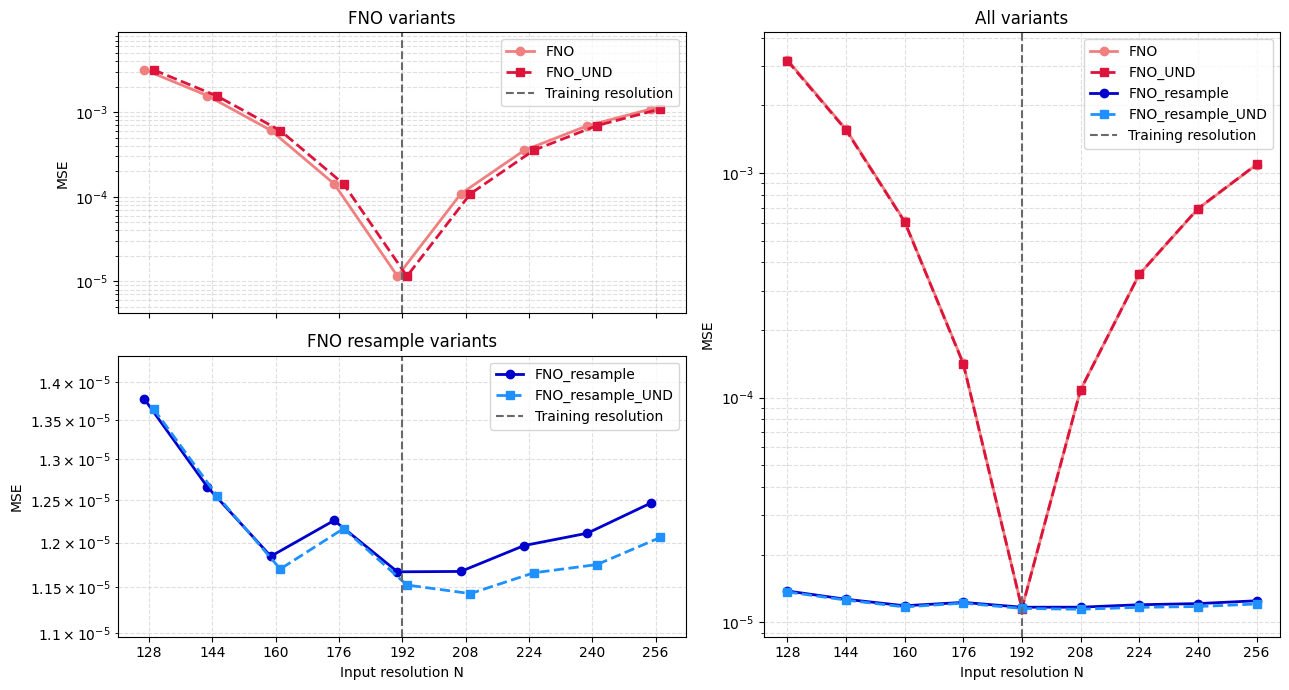
\includegraphics[width=0.8\textwidth]{figures/improving_fno.png}
    \caption{\label{fig:improving-fno} MSE loss as a function of evaluation resolution for four FNO variants trained on the Navier--Stokes dataset. The left panels separate the nearly overlapping curves for readability: the top panel compares the standard FNO and FNO\_UND, while the bottom panel compares FNO\_resample and FNO\_resample\_UND. A small horizontal offset is applied to the curves in these two panels only to make both models visible. The right panel shows all four variants on the same axes without offset. The vertical dashed lines mark the training resolution.
}
\end{figure}

The previous section identified resolution-dependent internal representations as the main source of poor resolution transfer in the standard FNO. In particular, the layerwise diagnostic in Figure~\ref{fig:fno_internal_drift} showed that the internal representation changes sharply after fixed-cell padding. This suggests that the FNO may benefit from the same fixed-grid strategy used in the CNO, where the main learned operator is applied on a consistent internal discretization rather than directly on the input grid.

To test this, two modifications inspired by the CNO were added to the FNO. The first is fixed-grid resampling, where all inputs are first resampled onto the training resolution before being passed through the FNO. The second is the UND block, which is designed to reduce aliasing introduced by nonlinear activations. These modifications were tested separately and in combination, giving four models: the standard FNO, FNO\_UND, FNO\_resample, and FNO\_resample\_UND. All four models retained 16 Fourier modes in each direction and were trained and evaluated on the Navier--Stokes dataset.

\begin{table}
    \centering
    \caption{\label{tab:d-values-navier-stokes-improved-fno} Values of \(D\) for the modified FNO models on the Navier--Stokes dataset. Lower values of \(D\) indicate more consistent loss across evaluation resolutions.}
    \begin{tabular}{lc}
        \hline
        Model & \(D\) \\
        \hline
        FNO & 3.4817 \\
        FNO\_UND & 3.4800 \\
        FNO\_resample & 0.0490 \\
        FNO\_resample\_UND & 0.0456 \\
        \hline
    \end{tabular}
\end{table}

The results are shown in Figure~\ref{fig:improving-fno}, with the corresponding values of \(D\) reported in Table~\ref{tab:d-values-navier-stokes-improved-fno}. Adding the UND block alone produces almost no change. The value of \(D\) changes from 3.4817 for the standard FNO to 3.4800 for FNO\_UND, indicating that nonlinear aliasing from the activation functions is not the dominant source of the observed resolution dependence.

In contrast, fixed-grid resampling produces a large improvement. FNO\_resample reduces \(D\) from 3.4817 to 0.0490, while FNO\_resample\_UND gives a similar value of 0.0456. This supports the interpretation developed in Section~\ref{sec:fno_discussion}: the main issue is not the Fourier basis alone, nor simply the finite number of retained modes, but the fact that the standard FNO executes its learned computation on the evaluation grid. When the evaluation resolution changes, the coordinate representation, padding operation, Fourier transforms, and spectral weights are applied to a different internal representation than the one seen during training.

Fixed-grid resampling avoids this by ensuring that the FNO layers are always applied at the same internal resolution. In particular, the fixed-cell padding is then applied after the input has been mapped to the training resolution, so the padded region has the same physical meaning during training and evaluation. This removes the dominant source of internal representation drift identified in Figure~\ref{fig:fno_internal_drift}.

The small additional improvement from combining resampling with the UND block suggests that aliasing from nonlinear activations may still contribute slightly once the dominant representation mismatch has been removed. However, the difference between FNO\_resample and FNO\_resample\_UND is minor compared with the improvement caused by fixed-grid resampling itself.

These results show that the poor discretization robustness of the standard FNO is strongly linked to the fixed-cell padding operation. When the model is evaluated directly at a different spatial resolution, the same number of padded cells corresponds to a different physical padding width than during training. Mapping all inputs to the training resolution before applying the FNO removes this padding mismatch, so the Fourier layers and padding operation act on the same internal representation during both training and inference.
\chapter{Non-Uniform Meshes -- Results and Discussion} \label{cha:non-uniform-results-discussion}

\section{Results}

\subsection{Incompressible Navier-Stokes flow past a cylinder}

\begin{figure}
    \centering
    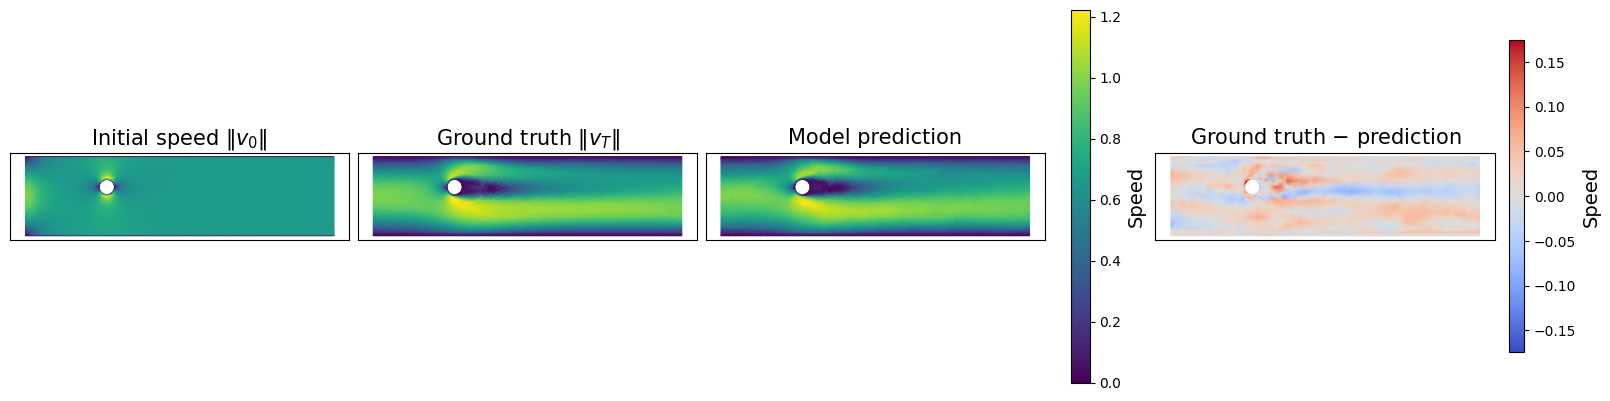
\includegraphics[width=0.99\textwidth]{figures/cylinder_flow_prediction_difference.png}
    \caption{\label{fig:geo-fno-cylinder-result}
    Representative Geo-FNO prediction on the cylinder flow dataset. The model predicts the horizontal and vertical velocity components separately; for visualization, the panels show the corresponding speed \(\|\mathbf{v}\|\). The panels show the initial speed field, the ground-truth final speed field, the model prediction, and the pointwise difference between prediction and ground truth on the irregular spatial mesh.}
\end{figure}

The Geo-FNO was first evaluated on the cylinder flow dataset. Figure~\ref{fig:geo-fno-cylinder-result} shows a representative prediction on a held-out test sample. Across the test set, the model reached an MSE of \(4.733\times10^{-3}\).

The prediction captures the main structure of the final velocity field, including the global flow pattern around the cylinder and the downstream wake. The difference plot shows that the error is not distributed uniformly across the domain. Larger errors occur primarily in regions where the velocity field changes more sharply, especially near the wake and around the obstacle. Despite these local errors, the qualitative agreement between the prediction and the ground truth indicates that Geo-FNO can learn the velocity-field mapping directly on the irregular point-cloud representation.

\subsection{HTGR column temperature dataset}

\begin{figure}
    \centering
    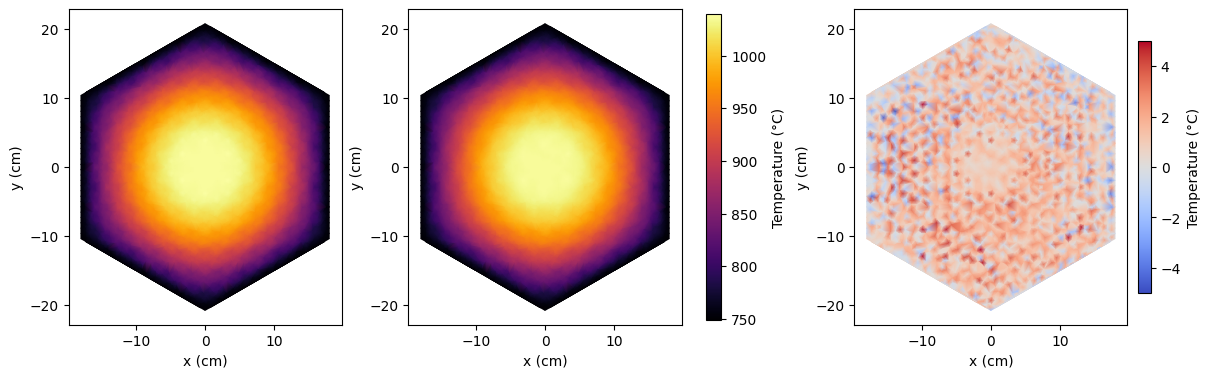
\includegraphics[width=1\textwidth]{figures/htgr_trigonometric_pred.png}
    \caption{\label{fig:geo-fno-htgr-result}
    Representative Geo-FNO prediction on the HTGR column temperature dataset. The panels show the ground-truth temperature field, the model prediction, and the signed difference between prediction and ground truth on the irregular spatial mesh. This sample corresponds to an axial level of \(z=30\,\mathrm{cm}\) and a boundary temperature of \(T=750\,^{\circ}\mathrm{C}\).}
\end{figure}

\begin{figure}
    \centering
    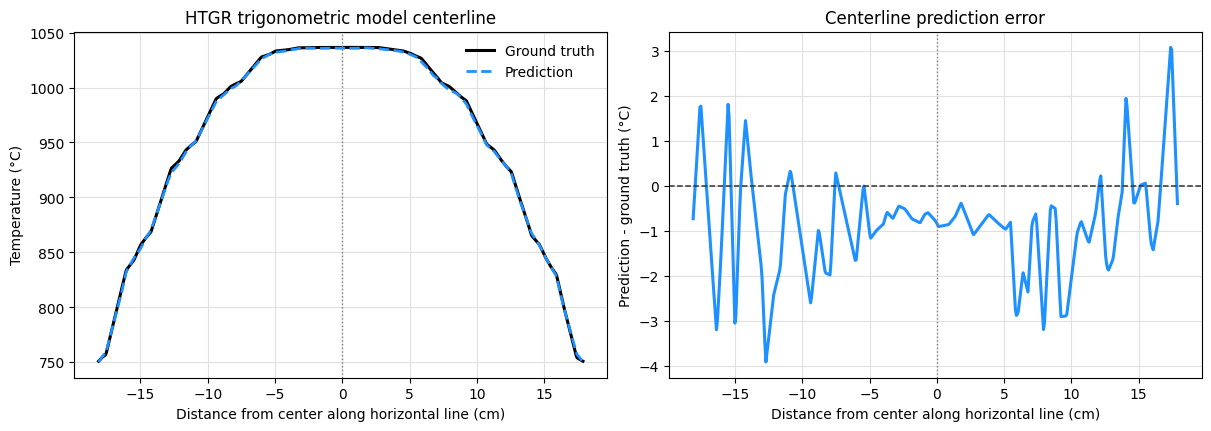
\includegraphics[width=0.9\textwidth]{figures/htgr_centerline.png}
    \caption{\label{fig:htgr-centerline}
    Horizontal centerline comparison for the HTGR sample shown in Figure~\ref{fig:geo-fno-htgr-result}. The left panel compares the ground-truth and predicted temperature profiles along the centerline, while the right panel shows the signed error \(T_{\mathrm{pred}}-T_{\mathrm{true}}\). The profile confirms that the model reproduces the temperature fall-off from the hot central region toward the cooler boundary, with remaining centerline errors of only a few degrees Celsius.}
\end{figure}

The Geo\hyp{}FNO was evaluated on the HTGR column temperature dataset described in Section~\ref{htgr-column-dataset}. Figure~\ref{fig:geo-fno-htgr-result} shows a representative prediction on a held\hyp{}out sample. Across the test set, the model reached an MSE of \(2.18\), corresponding to a relative RMSE of \(2.07\times10^{-3}\).

The predicted temperature field closely matches the ground truth. The dominant spatial temperature pattern is reproduced, with a hot central region and lower temperatures near the boundary. The difference plot shows local deviations of only a few degrees Celsius relative to an overall temperature range of several hundred degrees.

To examine whether the model reproduces the temperature fall-off from the center toward the boundary, a horizontal centerline profile was extracted from the same sample. Figure~\ref{fig:htgr-centerline} shows that the predicted and ground-truth profiles are nearly indistinguishable on the full temperature scale. The signed error remains within a few degrees Celsius along the profile, indicating that the apparent differences in the two-dimensional error plot are small local deviations rather than a substantial systematic error in the center-to-boundary temperature profile.




\section{Discussion}

\subsection{Incompressible Navier-Stokes Flow Past a Cylinder}

The cylinder flow dataset provides a challenging benchmark for mesh-free operator learning because the model must learn nontrivial fluid dynamics on a geometry that changes between samples. The cylinder radius and position vary across the dataset, and the solution is represented on a non-uniform point cloud rather than on a fixed Cartesian grid. The task is therefore not only to predict the velocity field, but also to do so across changing geometries and irregular sampling patterns.

Since the inlet speed and viscosity are fixed across the dataset, the Reynolds number varies directly with the cylinder radius,
\begin{equation}
Re = \frac{2UR}{\nu},
\end{equation}
where \(U\) is the inlet speed, \(R\) is the cylinder radius, and \(\nu\) is the kinematic viscosity \cite{cylinder-flow-re}. Larger cylinders therefore correspond to higher Reynolds numbers. For flow past a circular cylinder, periodic vortex shedding is expected above a critical Reynolds number of approximately \(Re\approx47\) \cite{cylinder-wake}, which provides a useful reference point for interpreting the prediction errors. Vortex shedding refers to the periodic formation and detachment of alternating vortices from opposite sides of the cylinder, resulting in oscillatory downstream wake behavior.

Figure~\ref{fig:cylinder-loss-re} shows the relative \(L^2\) velocity loss as a function of Reynolds number on the test set. The loss is elevated for the smallest cylinders, decreases for intermediate Reynolds numbers, and then increases gradually above the expected vortex-shedding onset. This suggests that the higher-\(Re\) samples are more difficult at least partly because the wake becomes increasingly unsteady. 

In this regime, the final state is not characterized only by a mean downstream wake shape, but also by the instantaneous position and phase of the wake structures. This makes the one-shot prediction task substantially harder. Vortex shedding does not begin immediately at the initial time of the prediction; the flow must first interact with the cylinder, the separated wake must develop, and the onset time and subsequent phase depend on the geometry and flow evolution. A model that maps directly from the initial state to the final state must therefore infer both the development of the oscillatory wake and its final phase without explicitly resolving the intermediate dynamics. Small errors in the inferred onset, frequency, or accumulated phase can place the wake displacement on the wrong side of the centerline, producing a large pointwise \(L^2\) error even when the predicted wake is qualitatively reasonable. This helps explain why the model tends to predict a smoother wake structure in the higher-\(Re\) cases.

\begin{figure}
    \centering
    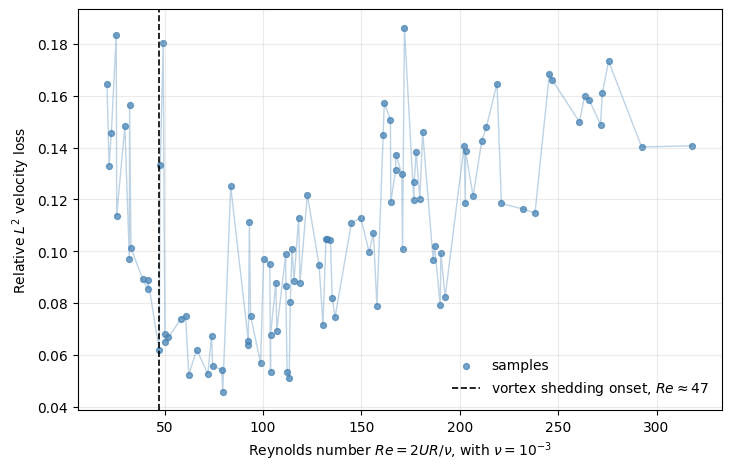
\includegraphics[width=0.8\textwidth]{figures/cylinder_flow_loss_vs_re.png}
    \caption{\label{fig:cylinder-loss-re}
    Relative \(L^2\) velocity loss for Geo-FNO on the cylinder flow test set as a function of Reynolds number \(Re=2UR/\nu\). Since \(U\) and \(\nu\) are fixed in the dataset, \(Re\) varies directly with the cylinder radius. The vertical dashed line marks the approximate onset of vortex shedding for flow past a circular cylinder, \(Re\approx47\).}
\end{figure}

This behavior is illustrated in Figure~\ref{fig:geo-fno-cylinder-result-unsteady}. The model captures the global flow around the cylinder and the approximate wake location, but the downstream wake in the prediction is smoother than in the ground truth. The resulting error is concentrated in the wake region, where small differences in the instantaneous wake structure are heavily penalized by the pointwise loss. This supports the interpretation that a significant part of the remaining error is associated with predicting detailed wake structure rather than with a failure to learn the dominant flow response.

\begin{figure}
    \centering
    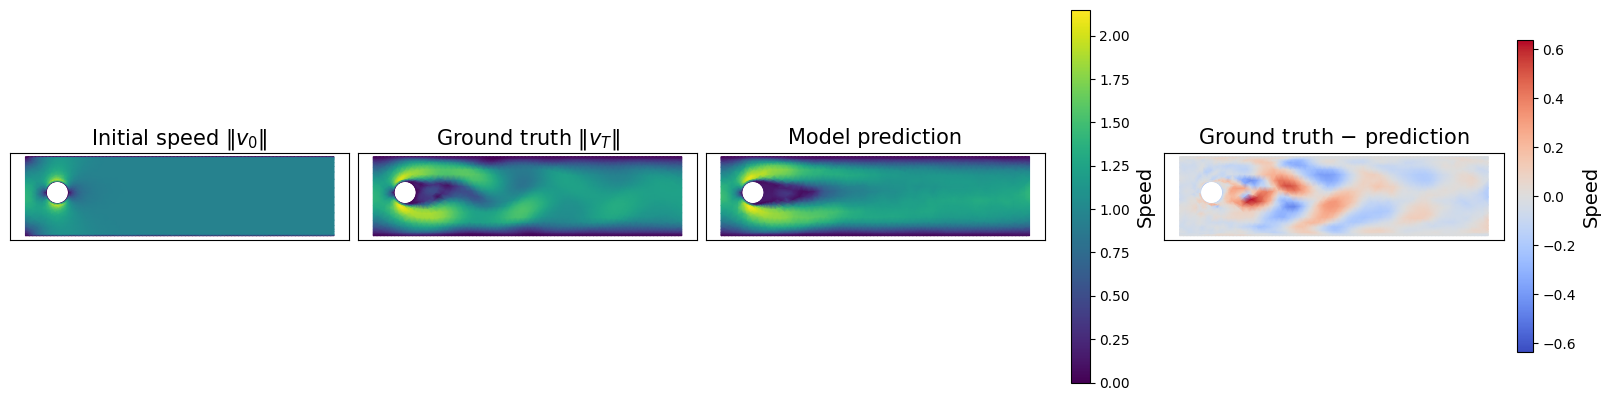
\includegraphics[width=0.99\textwidth]{figures/cylinder_flow_prediction_no_steady_state.png}
    \caption{\label{fig:geo-fno-cylinder-result-unsteady}
    Geo-FNO prediction on a cylinder flow sample with an oscillatory downstream wake. The model predicts the horizontal and vertical velocity components separately; for visualization, the panels show the corresponding speed \(\|\mathbf{v}\|\). The model captures the global flow structure but predicts a smoother wake than the ground truth, leading to larger localized errors downstream of the cylinder.}
\end{figure}

The elevated losses at the smallest Reynolds numbers are not explained by wake instability. These samples correspond to the smallest cylinders, where the obstacle boundary is represented by fewer mesh points and the near-cylinder disturbance occupies a smaller region of the point cloud. Small errors near the obstacle or in the immediate wake may therefore have a larger effect on the relative velocity loss. This remains a hypothesis, since no separate mesh-resolution diagnostic was performed for the small-radius cases.

Overall, Geo-FNO learns the dominant flow response across changing cylinder geometries, but the remaining errors concentrate in regimes where the final state is sensitive to small geometric or dynamical changes. The Reynolds-number trend points to wake instability as a major contributor at high \(Re\), while the small-radius errors may reflect the difficulty of representing very small obstacles on the irregular point cloud. The model can therefore learn the global flow response directly on a non-uniform mesh, but detailed one-shot prediction of sensitive wake structures remains challenging.

\subsection{HTGR Column Temperature Dataset}

The strong performance of Geo-FNO on the HTGR column temperature dataset should be interpreted in the context of the structure of the task. Compared to the cylinder flow benchmark, this problem is smoother and lower-dimensional. The output field is a scalar temperature distribution rather than a vector-valued velocity field, and the dominant physical behavior is governed by diffusion and heat transport rather than strongly nonlinear wake dynamics.

In addition, the spatial mesh is shared across all samples. Unlike the cylinder flow dataset, where both the geometry and the point cloud vary between samples, Geo-FNO is always evaluated on the same underlying irregular mesh. The model therefore does not need to adapt to changing geometries or different point distributions, and the challenge is focused primarily on learning the temperature field itself rather than learning across varying spatial representations.

The input space is also significantly simpler. As described in Section~\ref{htgr-column-dataset}, the prediction depends only on the boundary temperature and the axial position of the slice\footnote{As discussed in Appendix~\ref{appendix:htgr-input-engineering}, a trigonometric representation of \(z\) and \(T\) produced the lowest loss and was therefore used for the results reported here.}. This makes the task closer to learning a smooth parametric family of temperature fields than to solving a fully general operator learning problem with high-dimensional functional inputs.

Figure~\ref{fig:geo-fno-htgr-result} shows that Geo-FNO reproduces the dominant temperature structure accurately. The prediction captures the hot central region and the decrease toward the cooler boundary, while the difference plot shows only small local deviations relative to the overall temperature scale. To check whether the model reproduces the temperature fall-off from the center to the boundary, a horizontal centerline profile was extracted from the same sample. Figure~\ref{fig:htgr-centerline} shows that the predicted and ground-truth profiles are nearly indistinguishable on the full temperature scale. The signed error remains within a few degrees Celsius along the profile, indicating that the apparent differences in the two-dimensional error plot are small local deviations rather than a substantial systematic error in the center-to-boundary temperature profile.

These results show that Geo-FNO can be applied successfully to reactor-relevant temperature fields defined on non-uniform meshes without requiring interpolation onto a uniform Cartesian grid. This is useful in practice, since reactor geometries often involve curved boundaries and spatial layouts that are not naturally represented on regular grids.

At the same time, the relative simplicity of the HTGR task should be kept in mind. Because the geometry is fixed, the field is smooth, and the input space is low-dimensional, this experiment is best interpreted as a proof of applicability rather than a demonstration of performance on more complex reactor simulations. It shows that Geo-FNO can operate effectively on irregular reactor meshes, but does not by itself establish performance on fully general multiphysics reactor problems.

\subsection{Interpretation of Discretization Invariance on Mesh-Free Grids}

Section~\ref{mesh-free-discretization-invariance} explained that mesh-free discretization robustness requires comparing predictions for the same underlying physical sample across systematically varied point-cloud or mesh representations. The Geo-FNO experiments in this chapter do not provide such a controlled refinement study. Instead, they test whether Geo-FNO can learn directly on the irregular spatial representations available in the two datasets.

The cylinder flow dataset is the closer of the two to a mesh-free generalization test, because both the geometry and the point cloud vary between samples. However, these variations are coupled: changing the cylinder radius or position also changes the physical flow problem. As a result, the experiment tests generalization across geometries and irregular point clouds, but it does not isolate the effect of changing the discretization of one fixed physical sample.

The HTGR dataset has the opposite limitation. The spatial mesh is irregular, but it is shared across all samples. The experiment therefore shows that Geo-FNO can learn accurate temperature fields on a fixed irregular reactor mesh, but it does not test robustness to changes in mesh density, element size, or point placement.

The results should therefore be interpreted as evidence of applicability to irregular spatial representations rather than as a direct demonstration of mesh-free discretization invariance. A full test would require controlled families of meshes or point clouds for the same physical states, as discussed in Section~\ref{mesh-free-discretization-invariance}.
\chapter{\label{cha:conclusion}Conclusions and Future Work}

\section{Conclusions}

A central finding from the uniform-grid experiments is that the poor resolution transfer of the tested FNO is mainly caused by fixed-cell spatial padding, not by the Fourier basis alone. The FNO can achieve very low error at the training resolution, but the diagnostics in Section~\ref{sec:fno_diagnostics} show that its retained-mode representation changes substantially when the same model is evaluated on a different spatial grid. In particular, the layerwise drift diagnostic in Figure~\ref{fig:fno_internal_drift} shows that fixed-cell padding introduces the first large resolution-dependent divergence from the training-resolution forward pass. The reason is that a fixed number of padded cells corresponds to a different fraction of the physical domain when the spatial resolution changes. The fixed-grid FNO experiment in Section~\ref{sec:improving_fno} supports this interpretation: mapping all input resolutions to the training resolution makes the padding operation physically consistent again and reduces \(D\) by nearly two orders of magnitude.

The CNO results show that controlling the internal representation improves resolution robustness, but also introduces interpolation and bandlimit constraints. For a convolutional encoder--decoder, a fixed internal grid prevents the physical scale of the learned kernels from changing when the input resolution changes, which explains the much flatter CNO loss curves as seen in Figures~\ref{fig:loss_vs_resolution_navier_stokes} and \ref{fig:loss_vs_resolution_darcy_flow}. However, the model then always predicts through a chosen internal resolution, so the result depends on interpolation and on the bandlimit imposed by that grid. The UND block adds further representation control by reducing nonlinear aliasing, but its empirical role is nuanced: it improves performance on Darcy flow, while CNO\_no\_UND slightly outperforms the standard CNO at high Navier--Stokes resolutions. The results therefore point to a trade-off between representation consistency and finite-grid predictive accuracy.

For non-uniform meshes, the Geo-FNO experiments show that Fourier-based operator learning can be applied directly to irregular point-cloud data. The model produced meaningful predictions on both cylinder flow and HTGR temperature data without first interpolating onto a uniform Cartesian grid. These results demonstrate applicability to irregular spatial representations, but not mesh-free discretization invariance in the strict sense: the cylinder flow point clouds change together with the geometry, while the HTGR mesh is fixed across samples.

The cylinder flow results also show that the formulation of the prediction task matters. At higher Reynolds numbers, the loss increases and the largest errors occur in the downstream wake, where vortex shedding makes the final state sensitive to the instantaneous wake phase. Geo-FNO often captures the global flow pattern and approximate wake location, but smooths the detailed oscillatory wake. This suggests that part of the remaining error is tied to one-shot prediction of an unsteady process, not only to the spatial representation used by the model.

Overall, robust neural operator surrogates require the internal representation of the model to remain consistent with the physical problem being approximated. Fixed internal resolutions are one way to improve resolution transfer, but they introduce bandlimit and interpolation assumptions. Mesh\hyp{}free models avoid regular\hyp{}grid preprocessing, but their discretization robustness is best assessed using datasets designed for controlled changes in sampling geometry. For reactor modeling, both architecture design and dataset design are therefore central to making neural operators reliable surrogate models.

\section{Future Work}

Several natural extensions of this work remain for future study.

The most immediate follow-up is to test the role of padding in the FNO more directly. The layerwise diagnostics identified fixed-cell padding as the largest source of internal representation drift under resolution transfer. A clean first test would therefore be to repeat the resolution-transfer experiments on the same datasets with padding disabled, so that the FNO is evaluated without introducing an unnecessary padded extension of the domain. For non-periodic fields, the next step would be to test physically scaled padding. A modified implementation could instead specify the padding as a fixed fraction of the domain size, so that it has the same physical meaning across resolutions. Together, these experiments would test whether the standard FNO can recover much of the robustness obtained through fixed-grid resampling while avoiding the additional interpolation step.

A second important extension is a controlled study of discretization robustness on non-uniform meshes. Unlike the uniform-grid experiments, where changing \(N\) provides a simple refinement path, non-uniform meshes require the refinement strategy itself to be specified. Future datasets should therefore contain the same physical samples represented on families of related point clouds or meshes, with controlled changes in global point count, local sampling density, or element size. For example, one could refine sampling near cylinder boundaries, wake regions, thermal boundary layers, or material interfaces while keeping the underlying physical solution fixed. This would make it possible to distinguish true robustness to discretization changes from generalization across different geometries or input parameters.

A third priority is the use of more challenging non-uniform reactor datasets. The HTGR temperature experiment demonstrates that Geo-FNO can be applied to nuclear reactor data on an irregular mesh, but the problem itself is smooth, fixed-geometry, and low-dimensional. Future work should therefore consider datasets involving stronger nonlinear coupling and more complex physical behavior, such as transient thermal-hydraulics, coupled neutronics and heat transfer or spatially varying material properties. Such datasets would provide a more meaningful test of whether neural operators can function as practical surrogate models in reactor analysis.

Another limitation of the mesh-free experiments is that only Geo-FNO was evaluated. For the uniform-grid experiments, the comparison between FNO and CNO was essential for separating the effects of global and local inductive biases. For non-uniform meshes, a similar comparison is still needed. Future work should compare Geo-FNO against locally structured mesh-free models such as CALM-PDE\footnote{Abbreviation of Continuous and Adaptive Convolutions for Latent Space Modeling of Time-dependent PDEs.} \cite{calm-pde}, as well as against the baseline of interpolating the data onto a uniform Cartesian grid before applying a standard FNO or CNO. Such comparisons would help determine whether the advantages of Geo-FNO come primarily from learning directly on the original point cloud, from the learned coordinate transform, or from the spectral structure of the architecture.

A related architectural direction is the development of a geometry-aware Convolutional Neural Operator. One possible approach would be to combine the learned coordinate transformation \(\phi^{-1}\) from Geo-FNO with the CNO architecture by first mapping the irregular point cloud to a more regular computational representation and then applying a convolutional neural operator instead of an FNO. This could preserve the local inductive bias of convolutional models while retaining the fixed internal representation and bandlimiting ideas that were effective in the uniform-grid experiments. Such an architecture would be especially relevant for cylinder flow, where the largest errors occur in localized wake structures.

The cylinder flow results also suggest that arbitrary-time or short-step prediction should be investigated for unsteady problems. The largest errors occur in cases with oscillatory wakes, where the model often captures the global wake structure but not the instantaneous wake phase. A natural extension would be to train Geo-FNO to predict short time increments and then apply it autoregressively, as is common in learned physical simulators \cite{pfaff-datasets}. This could be done using standard rollout-based training strategies, such as teacher forcing, scheduled sampling, or training on multi-step prediction losses \cite{recurrent-neural-operators}. Testing such variants would show whether the wake errors observed here are better addressed by changing the temporal formulation rather than by changing only the spatial architecture.

Overall, the central challenge remains the construction of neural operators whose internal representations remain faithful to the underlying continuous problem across changing discretizations. The results of this thesis suggest that progress on this problem will require three ingredients: architectures with controlled internal representations, datasets designed to test discretization changes cleanly, and temporal formulations that match the way the surrogate model will be used in practice. 

% Include references cited only in the appendix while keeping the
% bibliography before the appendix.
\nocite{batchelor1967fluid,chorin1993fluid,chandler2013kolmogorov,vela2024kolmogorov}
\bibliographystyle{plainnat}
\bibliography{sections/references}

\appendix
\def\chaptername{Appendix}
\chapter{\label{cha:glossary}Glossary}

In this appendix we give an overview of frequently used terms and
abbreviations.

\begin{description}
\item[foo:] \ldots
\item [bar:] \ldots
\end{description}

\chapter{\label{navier-details}Navier-Stokes data generation details}

The velocity field is not part of the stored dataset or the prediction target. Instead, it is reconstructed from the vorticity during data generation in order to evaluate the nonlinear advection term, using the streamfunction relation

\begin{equation}
    -\Delta \psi = \omega, \qquad u = \nabla^\perp \psi.
\end{equation}

to talk about:
forcing term is a sinusoidal term (show form?)
viscosity is kept constant; what is the value? 1e-5
method of generation; randomly generate N kx, ky modes, multiply by gaussian envelope, real field constraint, inverse transform
\include{sections/requirements}


\end{document}
